\documentclass[10pt]{beamer}

% ==================== 1. PREAMBLE ====================
\usetheme{Madrid}
\usecolortheme{whale}

% Colors (Navy + Gold)
\definecolor{DIATNavy}{RGB}{27, 42, 74}
\definecolor{DIATGold}{RGB}{197, 165, 90}
\definecolor{BodyGray}{RGB}{51, 51, 51}

\setbeamercolor{palette primary}{bg=DIATNavy,fg=white}
\setbeamercolor{palette secondary}{bg=DIATNavy,fg=white}
\setbeamercolor{palette tertiary}{bg=DIATNavy,fg=white}
\setbeamercolor{titlelike}{parent=palette primary}
\setbeamercolor{structure}{fg=DIATNavy}
\setbeamercolor{item}{fg=DIATGold}

% Fonts
\usepackage{fontspec}
\usepackage{polyglossia}
\setmainlanguage{english}
\setotherlanguage{sanskrit}
\newfontfamily\devanagarifont{Noto Serif Devanagari}[Script=Devanagari]
\newcommand{\dev}[1]{{\devanagarifont #1}}

\usepackage{graphicx}
\usepackage{booktabs}
\usepackage{tikz}
\usepackage{multicol}

% Logo configuration
\logo{
\includegraphics[height=0.8cm]{../images/DIATlogo.png}}

% Title Metadata
\title[Sanskrit NER]{BYT5-Sanskrit with Balanced Regularization for Sanskrit Named Entity Recognition}
\subtitle{M.Tech Thesis Defense}
\author[Yogesh]{Yogesh (24-14-15) \\ \medskip \small Under the supervision of: \\ \small Dr. S.V.S.S.N.V.G. Krishna Murthy}
\institute[DIAT Pune]{Department of Applied Mathematics \\ Defence Institute of Advanced Technology, Pune}
\date{May 2026}

% Custom Footline for Thesis Page References
\def\tpage{}
\newcommand{\tp}[1]{\def\tpage{#1}}
\setbeamertemplate{footline}{
  \leavevmode%
  \hbox{%
  \begin{beamercolorbox}[wd=.333333\paperwidth,ht=2.25ex,dp=1ex,center]{author in head/foot}%
    \usebeamerfont{author in head/foot}\insertshortauthor
  \end{beamercolorbox}%
  \begin{beamercolorbox}[wd=.333333\paperwidth,ht=2.25ex,dp=1ex,center]{title in head/foot}%
    \usebeamerfont{title in head/foot}\insertshorttitle
  \end{beamercolorbox}%
  \begin{beamercolorbox}[wd=.333333\paperwidth,ht=2.25ex,dp=1ex,right]{date in head/foot}%
    \usebeamerfont{date in head/foot}\insertshortdate{}\hspace*{2em}
    \insertframenumber{} / \inserttotalframenumber\hspace*{2ex} 
    \ifx\tpage\empty\else\color{DIATGold!80}(Thesis p. \tpage)\fi\hspace*{2ex}
  \end{beamercolorbox}}%
  \vskip0pt%
}

% ==================== 2. START DOCUMENT ====================
\begin{document}

% Slide 1: Title Slide
\begin{frame}[plain]
    \titlepage
    \begin{center}
        
\includegraphics[height=1.5cm]{../images/DIATlogo.png}
    \end{center}
\end{frame}

% Slide 2: Motivation
\begin{frame}{Motivation: Why Sanskrit NLP Matters}
    \tp{1}
    \begin{itemize}
        \item \textbf{Rich Intellectual Tradition:} Philosophy, Medicine, Statecraft, Mathematics.
        \item \textbf{Scale \& Complexity:} \textit{Mahābhārata} (100k verses), \textit{Rāmāyaṇa}, Purāṇas.
        \item \textbf{Access Barrier:} Scholars struggle to navigate massive classical corpora.
        \item \textbf{Translation Loss:} Subtle meanings lost in modern language translations.
        \item \textbf{Need:} Direct computational access to source knowledge.
    \end{itemize}
    \vfill
    \note{Sanskrit contains profound knowledge. But even scholars struggle to navigate these massive texts. NER is a foundational step for structured knowledge extraction.}
\end{frame}

% Slide 3: Problem Statement
\begin{frame}{The Problem Statement}
    \tp{2}
    \begin{block}{The Core Problem}
        Lack of a reliable Sanskrit NER system that satisfies three critical requirements simultaneously.
    \end{block}
    \begin{itemize}
        \item \textbf{Existing Models:} Optimize for one goal while sacrificing others.
        \item \textbf{Catastrophic Forgetting:} Pure NER fine-tuning destroys core linguistic skills (Segmentation, Lemmatisation).
        \item \textbf{Silver Data Quality:} Prior work failed to correctly leverage the DCS Sembank.
    \end{itemize}
    \vfill
    \note{Previous systems optimize for only one requirement. Our thesis addresses the "sweet spot" in the middle.}
\end{frame}

% Slide 4: The Three Desiderata
\begin{frame}{The Three Desiderata (Core Framework)}
    \tp{3}
    %\rowcolors{1}{white}{DIATGold!10}
    \begin{tabular}{lp{8cm}}
        \toprule
        \textbf{Goal} & \textbf{Requirement} \\
        \midrule
        \textbf{D1: Performance} & High Micro-F1 on Mahānāma gold-standard benchmark. \\
        \textbf{D2: Capability} & Preserve Segmentation (85\%+) and Lemmatisation (93\%+). \\
        \textbf{D3: Generalization} & Meaningful transfer to unseen classical texts (Pañcatantra). \\
        \bottomrule
    \end{tabular}
    \vfill
    \begin{itemize}
        \item These reflect \textbf{real-world scholarly needs}.
        \item Not just technical metrics, but functional utility targets.
    \end{itemize}
    \note{D1, D2, and D3 are our non-negotiable targets. D2 is especially important for scholars who need to analyze text grammar alongside entities.}
\end{frame}

% Slide 5: Contributions of This Thesis
\begin{frame}{Contributions of This Thesis}
    \tp{4}
    \begin{enumerate}
        \item \textbf{Novel DCS Sembank Extraction:} First correct pipeline yielding 12,955 clean examples.
        \item \textbf{Balanced Linguistic Regularisation:} 15\% multi-task ratio to prevent catastrophic forgetting.
        \item \textbf{3D Evaluation Framework:} Systematic comparison across D1, D2, and D3 dimensions.
        \item \textbf{ByT5-Sanskrit Validation:} Proving byte-level models handle Sanskrit morphology better.
    \end{enumerate}
    \vfill
    \begin{itemize}
        \item Result: \textbf{+16pp cross-domain gain} over Best NER baseline.
    \end{itemize}
    \note{Our methodology is the first to bridge the gap between high accuracy and linguistic preservation in Sanskrit NER.}
\end{frame}


% Slide 8: Chronological Literature Survey
\begin{frame}{Chronological Literature Survey}
    \tp{6}
    \centering
    \small
    \begin{tabular}{llp{7cm}}
        \toprule
        \textbf{Year} & \textbf{Authors} & \textbf{Paper / Contribution} \\
        \midrule
        1989 & McCloskey \& Cohen & Catastrophic Forgetting (Foundational Problem) \\
        1997 & Caruana & Multi-task Learning (Proposed Solution) \\
        2001 & Lafferty et al. & Conditional Random Fields (CRF Foundations) \\
        2015 & Huang et al. & BiLSTM-CRF for sequence tagging \\
        2018 & Hellwig \& Nehrdich & Sanskrit Character-level Segmentation \\
        2019 & Devlin et al. & BERT (Transformer Encoder) \\
        2022 & Xue et al. & ByT5 (Token-free byte-level modeling) \\
        2023 & Sarkar et al. & First Sanskrit NER attempt (CRF-based) \\
        2023 & Dettmers et al. & QLoRA (Efficient fine-tuning) \\
        2024 & Nehrdich et al. & \textbf{ByT5-Sanskrit} (One model is all you need) \\
        2025 & Sarkar et al. & \textbf{Mahānāma} (Gold-standard NER corpus) \\
        2025 & Hellwig \& Biagetti & Sanskrit Sembank (Relational extraction source) \\
        \bottomrule
    \end{tabular}
    \vfill
    \note{This timeline shows the progression from the 1989 discovery of catastrophic forgetting to our 2026 solution using the 2025 datasets.}
\end{frame}

% Slide 8: Research Gap
\begin{frame}{Identifying the Research Gap}
    \tp{7}
    \begin{itemize}
        \item \textbf{Missing Synergy:} No prior work addresses accuracy + linguistic skills + generalization.
        \item \textbf{Silver Data Bias:} DCS Sembank remained an "untapped" but noisy resource.
        \item \textbf{Model Dilution:} Multi-task models (M4) often sacrifice NER accuracy too much.
    \end{itemize}
    \vfill
    \begin{table}
        \centering
        \begin{tabular}{lccc}
            \toprule
            \textbf{Feature} & \textbf{Prev. Work} & \textbf{This Thesis} \\
            \midrule
            Gold NER (66k+ sents) & $\checkmark$ & $\checkmark$ \\
            Clean DCS Silver NER & $\times$ & $\checkmark$ \\
            Linguistic Regularization & $\times$ & $\checkmark$ \\
            Cross-Domain Eval (D3) & Limited & Rigorous \\
            \bottomrule
        \end{tabular}
    \end{table}
    \note{The key gap is the loss of segmentation and lemmatisation when fine-tuning. We fill this gap.}
\end{frame}

% Slide 8: Section Divider - Datasets
\begin{frame}[plain]
    \tp{8}
    \begin{center}
        \Huge \textbf{\color{DIATNavy}Dataset Description}
    \end{center}
\end{frame}

% Slide 9: The Four Pillar Datasets
\begin{frame}{The Four Pillar Datasets}
    \tp{9}
    \begin{table}
        \centering
        \small
        \begin{tabular}{llrl}
            \toprule
            \textbf{Dataset} & \textbf{Source} & \textbf{Sentences} & \textbf{Role in Thesis} \\
            \midrule
            \textbf{Mahānāma} & Sarkar et al. [2025] & 66,960 & Gold NER Training + D1 Eval \\
            \textbf{DCS Sembank} & Hellwig et al. [2025] & 18,855 & Silver NER Training \\
            \textbf{UD-Vedic} & Hellwig et al. [2020] & 27,182 & Linguistic Reg. (D2) \\
            \textbf{UD-UFAL} & Zeman et al. [2023] & 230 & Cross-Domain Eval (D3) \\
            \midrule
            \textbf{Total} & & \textbf{113,227} & \\
            \bottomrule
        \end{tabular}
    \end{table}
    \vfill
    \begin{itemize}
        \item \textbf{Heterogeneous Source:} Combining gold-standard, silver-standard, and morphological data to satisfy the three desiderata.
    \end{itemize}
    \note{These four datasets are the foundation of our multi-task training strategy.}
\end{frame}

% Slide 10: Selection Rationale & Composition
\begin{frame}{Dataset Selection Rationales \& Data Composition}
    \tp{10}
    \begin{columns}
        \begin{column}{0.6\textwidth}
            \begin{block}{Five Selection Criteria}
                \begin{enumerate}
                    \item \textbf{Task Alignment:} Direct NER or morphological potential.
                    \item \textbf{Domain Relevance:} Focus on Classical/Vedic Sanskrit.
                    \item \textbf{Language Purity:} 100\% Sanskrit content.
                    \item \textbf{Annotation Quality:} Gold (Mahānāma) vs High-Silver (DCS).
                    \item \textbf{Resource Efficiency:} Highest scholarly impact.
                \end{enumerate}
            \end{block}
        \end{column}
        \begin{column}{0.4\textwidth}
            \begin{center}
                \textbf{Training Mix} \\
                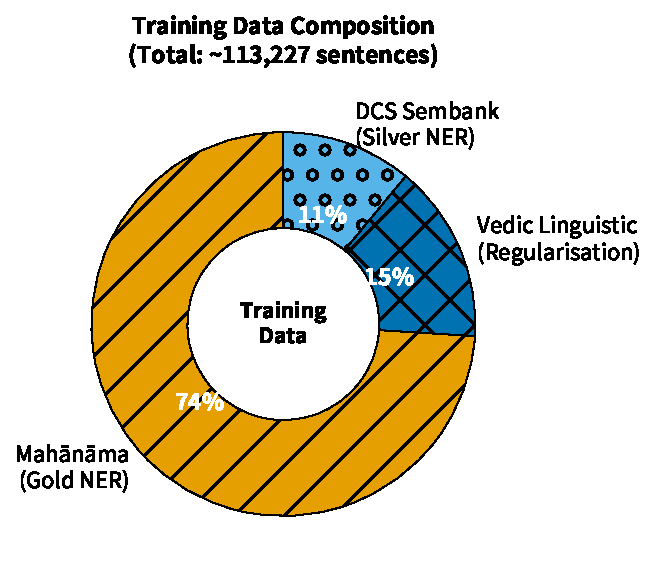
\includegraphics[width=\textwidth]{../figures/figure_3_3_training_data_composition.pdf}
            \end{center}
        \end{column}
    \end{columns}
    \vfill
    \begin{itemize}
        \item \textbf{Balanced Mix:} 74\% Gold NER, 11\% Silver NER, 15\% Morphological.
    \end{itemize}
\end{frame}

% Slide 11: Dataset Characteristics: The Imbalance Challenge
\begin{frame}{Dataset Characteristics: The Imbalance Challenge}
    \tp{11}
    \begin{columns}
        \begin{column}{0.5\textwidth}
            \begin{center}
                \textbf{Relative Data Sizes} \\
                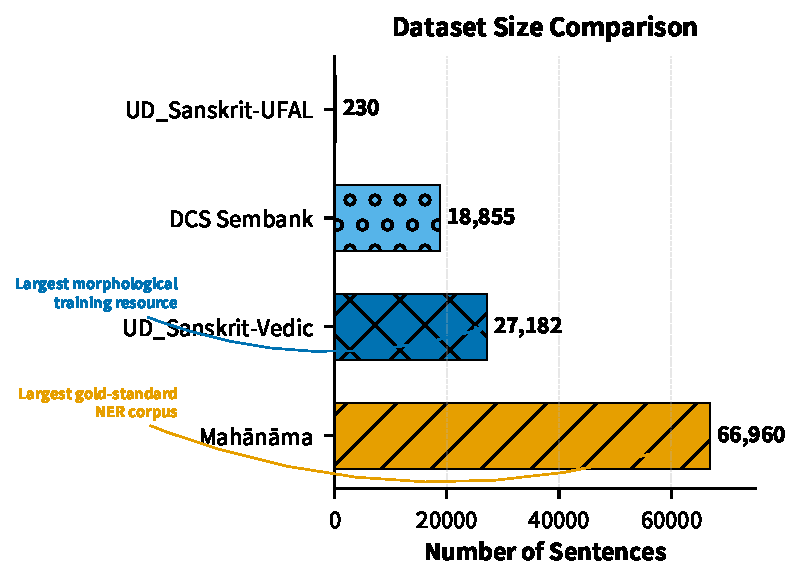
\includegraphics[width=\textwidth]{../figures/figure_3_1_dataset_size_comparison.pdf}
            \end{center}
        \end{column}
        \begin{column}{0.5\textwidth}
            \begin{center}
                \textbf{Entity Distribution (Gold)} \\
                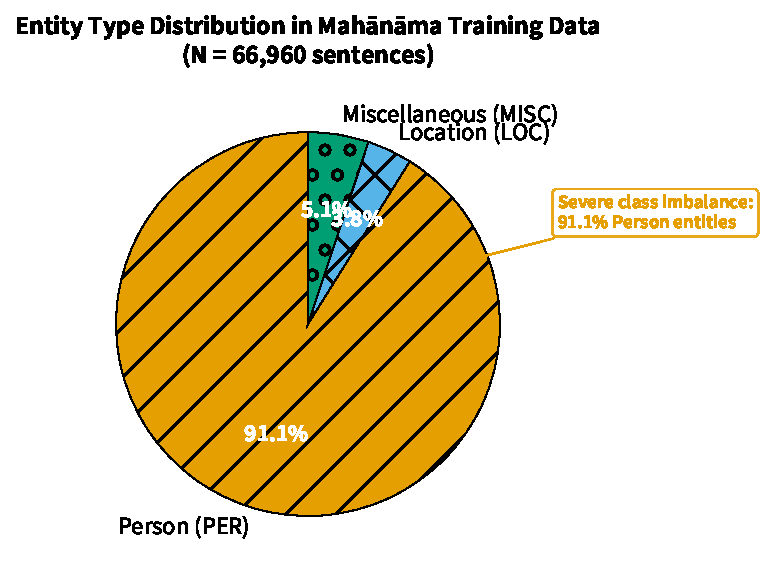
\includegraphics[width=\textwidth]{../figures/figure_3_2_mahanama_entity_distribution.pdf}
            \end{center}
        \end{column}
    \end{columns}
    \vfill
    \begin{itemize}
        \item \textbf{The 91\% PER Problem:} Mahānāma is heavily skewed towards Person entities.
        \item \textbf{Mitigation:} Oversampling LOC and MISC classes by 10x during training.
    \end{itemize}
\end{frame}

% Slide 12: Section Divider - Methodology
\begin{frame}[plain]
    \tp{12}
    \begin{center}
        \Huge \textbf{\color{DIATNavy}Methodology} \\
        \large The Core Technical Contributions
    \end{center}
\end{frame}

% Slide 13: Novel DCS Sembank Extraction (Concept)
\begin{frame}{Silver Data: DCS Sembank Integration}
    \tp{13}
    \begin{itemize}
        \item \textbf{DCS Sembank:} Lexical semantic resource mapping 600k+ words to synsets.
        \item \textbf{The Gap:} No explicit NER labels; semantic tags alone are insufficient.
        \item \textbf{Contribution:} Developed a deterministic extraction pipeline based on \textbf{Instance Relations}.
        \item \textbf{Logic:} If \texttt{col0\_id} (Descriptor) $\neq$ \texttt{col1\_id} (Proper Entity Name), we extract the substring as a silver NER example.
    \end{itemize}
    \vfill
    \begin{block}{Impact}
        Yielded 12,955 clean, diverse examples across 120 classical texts.
    \end{block}
\end{frame}

% Slide 14: DCS Extraction Pipeline (Visual)
\begin{frame}{DCS Sembank Extraction Pipeline}
    \tp{25}
    \begin{center}
        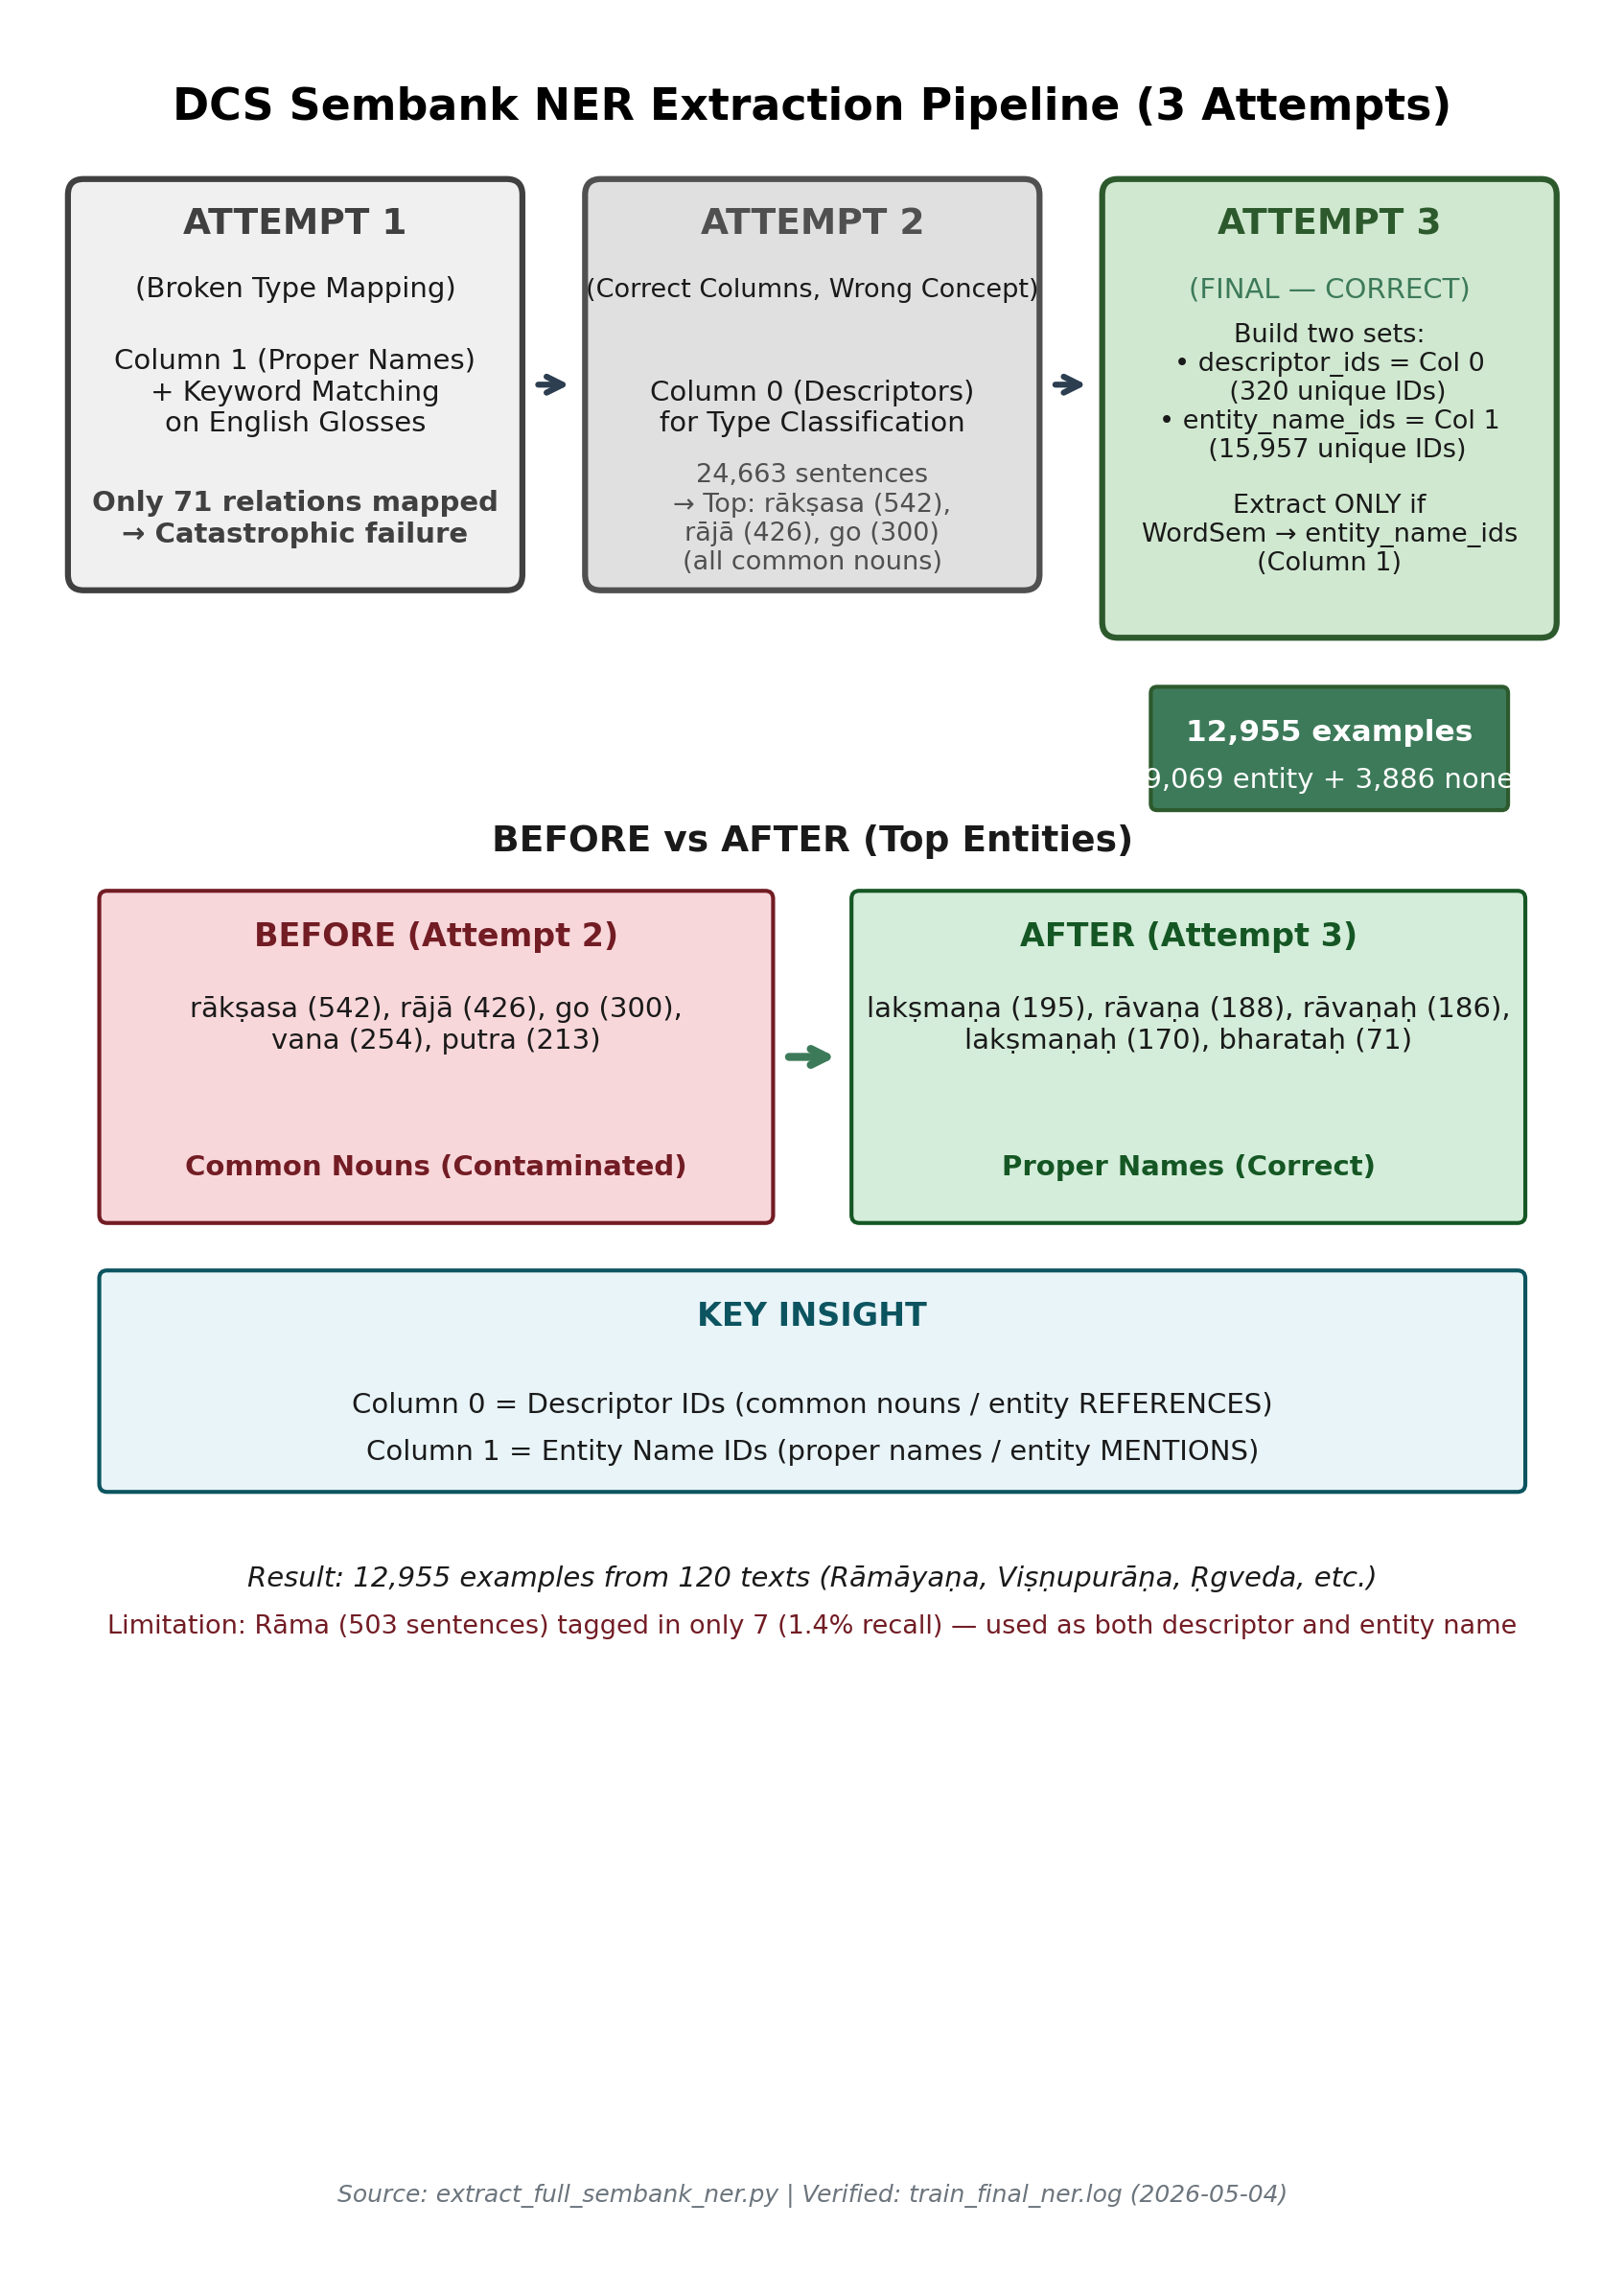
\includegraphics[height=0.85\textheight]{../figures/Figure_4_1_DCS_Extraction_Pipeline.png}
    \end{center}
    \note{The pipeline visualizes the journey from raw Sembank relations to clean, formatted NER pairs.}
\end{frame}

% Slide 15: Before vs After Extraction: Eliminating Noise
\begin{frame}{Before vs After Extraction: Eliminating Noise}
    \tp{25}
    \begin{columns}
        \begin{column}{0.5\textwidth}
            \begin{block}{Attempt 2 (Noisy)}
                \textbf{Top "Entities":} \\
                1. \dev{राक्षस} (rākṣasa) \\
                2. \dev{राजा} (rājā) \\
                3. \dev{गो} (go) \\
                \textit{Result: Common Noun contamination.}
            \end{block}
        \end{column}
        \begin{column}{0.5\textwidth}
            \begin{block}{Attempt 3 (Final)}
                \textbf{Top Entities:} \\
                1. lakṣmaṇa (195) \\
                2. rāvaṇa (188) \\
                3. rāvaṇaḥ (186) \\
                \textit{Result: Genuine proper names.}
            \end{block}
        \end{column}
    \end{columns}
    \vfill
    \begin{alertblock}{Key Limitation}
        "Rāma" functions as both descriptor and name; recall is low in silver data but compensated by gold data.
    \end{alertblock}
\end{frame}

% Slide 16: Python Algorithm: DCS Sembank Extraction
\begin{frame}[fragile]{Python Algorithm: DCS Sembank Extraction}
    \tp{25}
\begin{block}{Attempt 3: Deterministic Filtering}
\begin{verbatim}
def extract_silver_ner(sembank_row):
    # col0 = descriptor (e.g. king)
    # col1 = entity name (e.g. Rama)
    if sembank_row['col0_id'] != sembank_row['col1_id']:
        entity_text = sembank_row['col1_text']
        label = "PROPN"
        return (entity_text, label)
    return None

# Result: 12,955 high-precision examples
\end{verbatim}
\end{block}
    \vfill
    \begin{itemize}
        \item Prevents contamination from common nouns (\textit{rājan, go, vana}).
        \item Preserves inflectional diversity seen in classical manuscripts.
    \end{itemize}
\end{frame}

% Slide 17: Balanced Training Strategy
\begin{frame}{Balanced Training Strategy}
    \tp{28}
    \begin{itemize}
        \item \textbf{Hybrid Composition:} 74\% Gold + 11\% Silver + 15\% Linguistic.
        \item \textbf{Strategy 2:} 15\% S+L tasks (Segmentation + Lemmatisation).
        \item \textbf{Strategy 4:} Optimised schedule (10 epochs, 500 warmup steps).
    \end{itemize}
    \vfill
    \begin{center}
        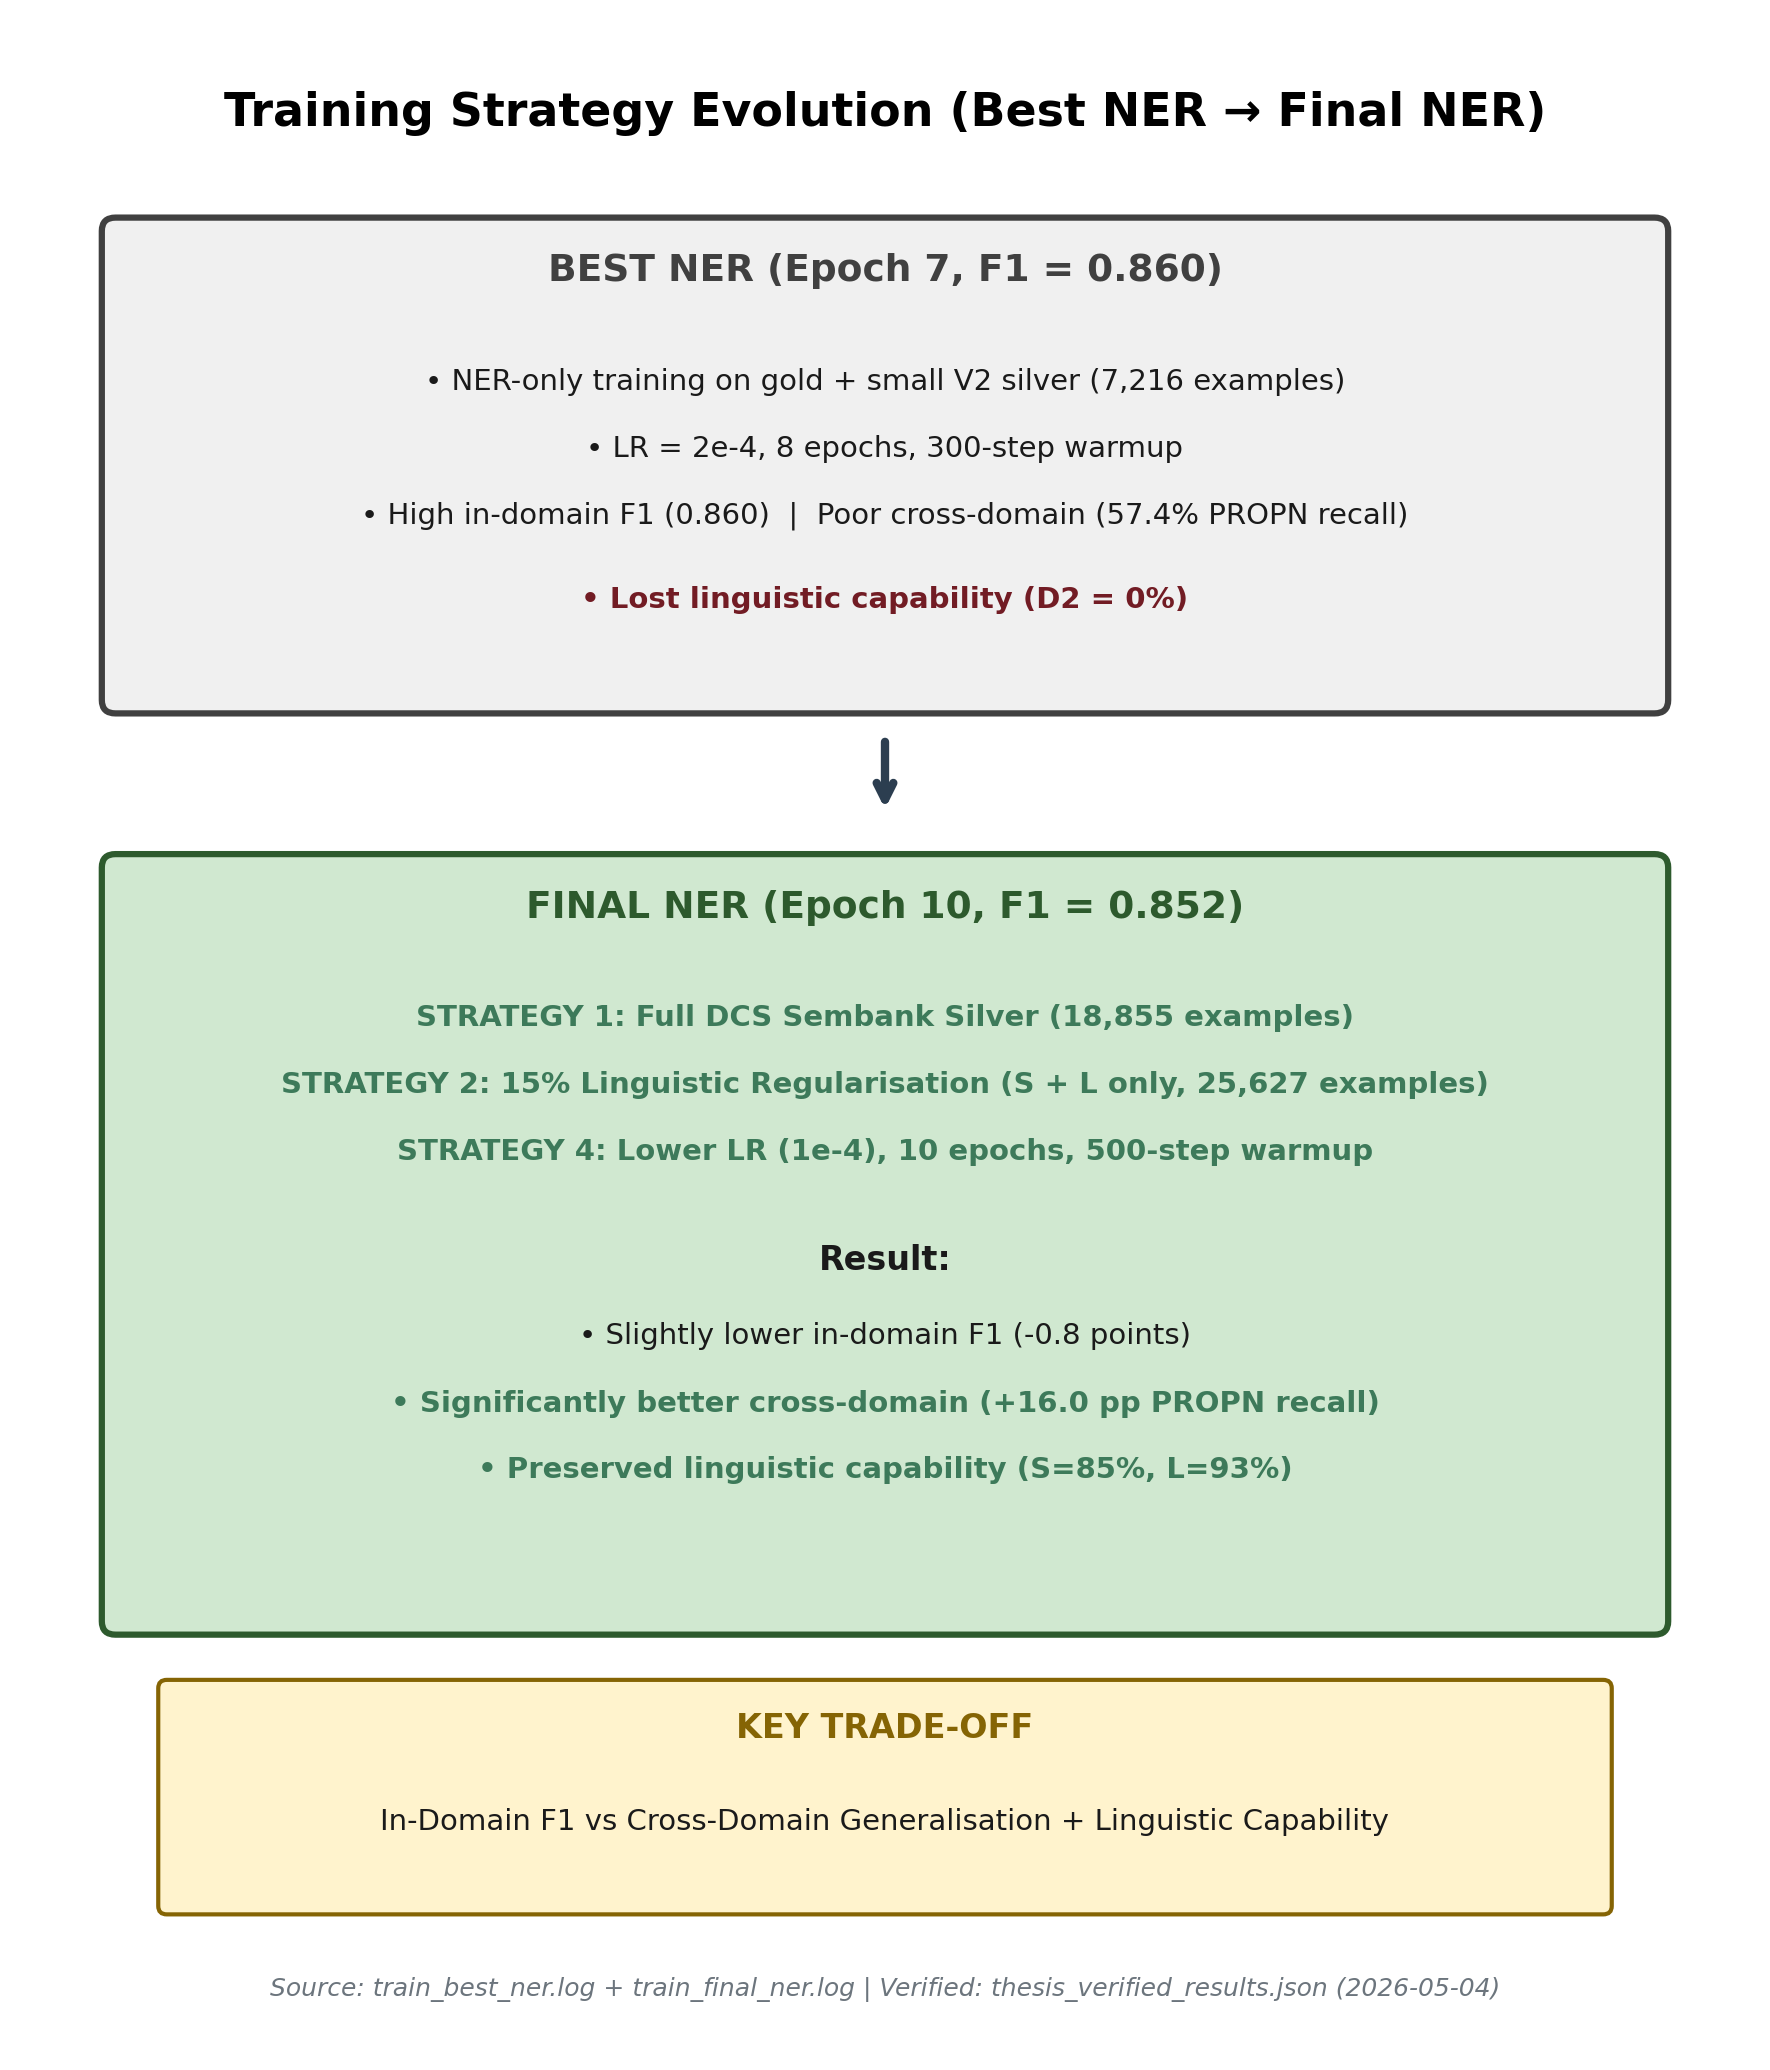
\includegraphics[height=0.55\textheight]{../figures/Figure_4_2_Training_Strategy_Evolution.png}
    \end{center}
    \note{The 15\% linguistic regularisation is our "secret sauce" that prevents the model from forgetting how to analyze Sanskrit while it learns to find entities.}
\end{frame}

% Slide 18: Why ByT5-Sanskrit? Architecture & Grounding
\begin{frame}{Why ByT5-Sanskrit? Architecture \& Grounding}
    \tp{29}
    \begin{columns}
        \begin{column}{0.6\textwidth}
            \begin{block}{Architecture: ByT5-Base (594M)}
                \begin{itemize}
                    \item \textbf{Encoder Layers:} 18
                    \item \textbf{Decoder Layers:} 6
                    \item \textbf{Rationale (3:1 Ratio):} 
                    \begin{itemize}
                        \item Deep encoder needed to extract semantic meaning from raw bytes.
                        \item Shallow decoder improves efficiency without performance loss.
                    \end{itemize}
                \end{itemize}
            \end{block}
            \begin{block}{Sanskrit Grounding}
                \begin{itemize}
                    \item \textbf{Pre-training:} 650k DCS sentences.
                    \item \textbf{Byte-Level:} Superior handling of Sandhi and complex compounding compared to subword models.
                \end{itemize}
            \end{block}
        \end{column}
        \begin{column}{0.4\textwidth}
            \begin{center}
                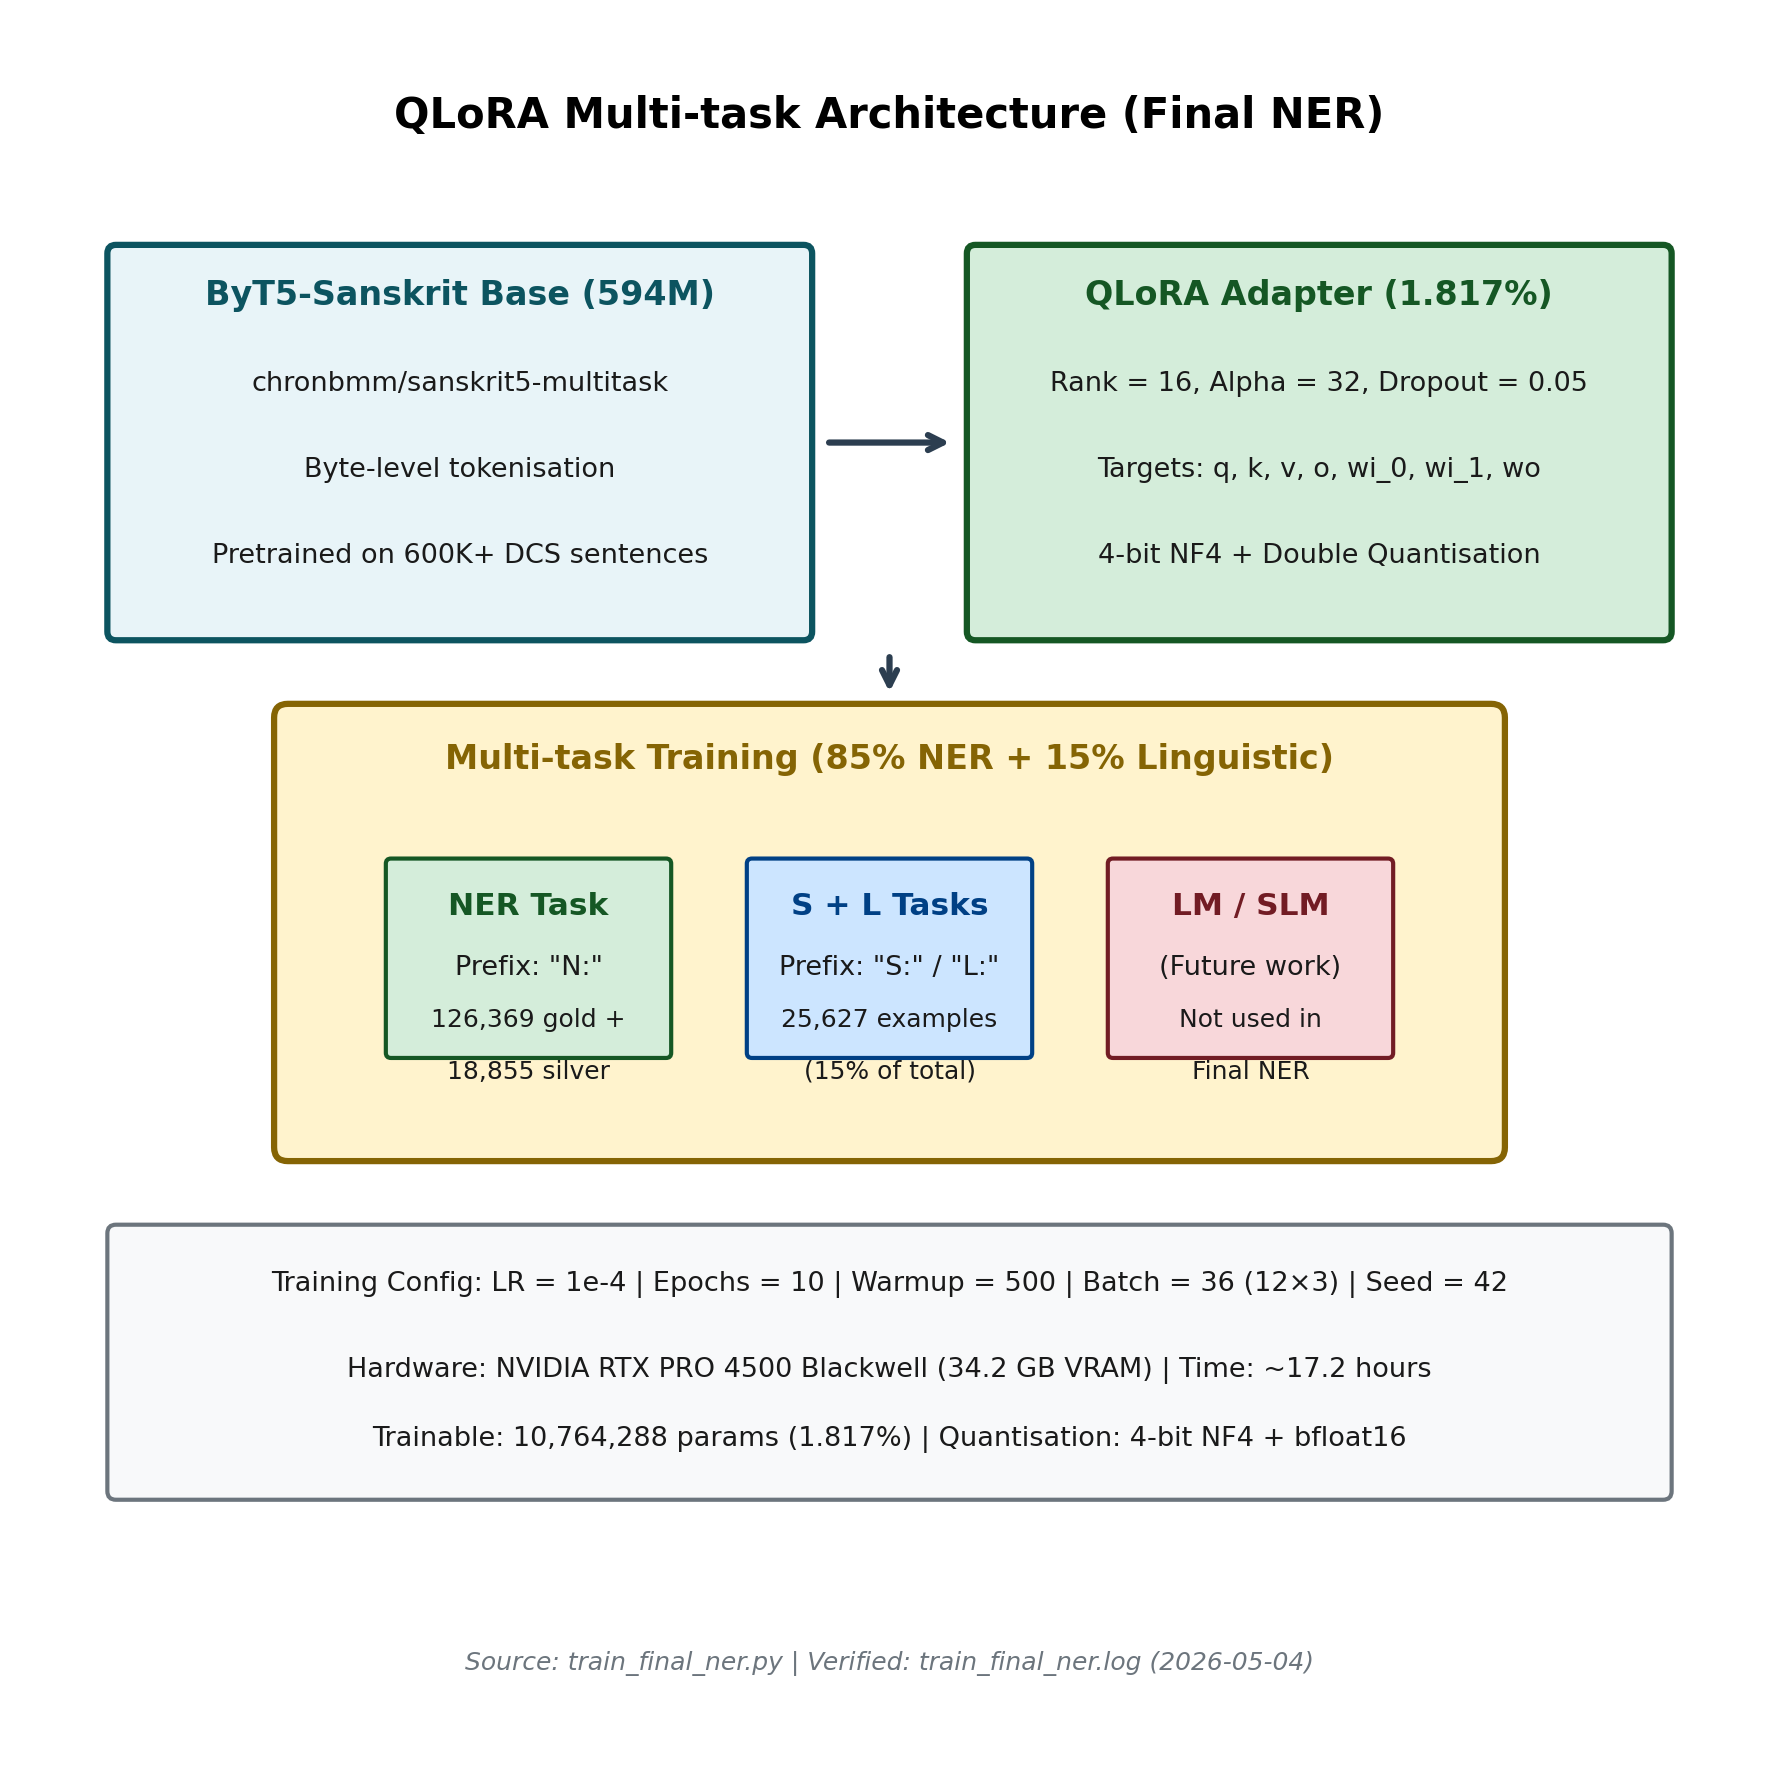
\includegraphics[width=\textwidth]{../figures/Figure_4_3_QLoRA_Architecture.png}
                \\ \scriptsize \textit{Final NER: 10.76M trainable params}
            \end{center}
        \end{column}
    \end{columns}
\end{frame}

% Slide 19: QLoRA Multi-task Architecture
\begin{frame}{QLoRA Multi-task Architecture}
    \tp{29}
    \begin{columns}
        \begin{column}{0.55\textwidth}
            \begin{itemize}
                \item \textbf{Base:} ByT5-Sanskrit (594M Parameters).
                \item \textbf{Quantization:} 4-bit NF4 with Double Quant.
                \item \textbf{PEFT:} QLoRA adapter (Rank=16, Alpha=32).
                \item \textbf{Trainable Params:} 10.76M (1.817\%).
            \end{itemize}
            \begin{block}{Machine Specifications}
                \begin{itemize}
                    \item \textbf{GPU:} NVIDIA RTX PRO 4500
                    \item \textbf{VRAM:} 34.2 GB
                    \item \textbf{Framework:} PyTorch 2.4 + Unsloth
                \end{itemize}
            \end{block}
        \end{column}
        \begin{column}{0.45\textwidth}
            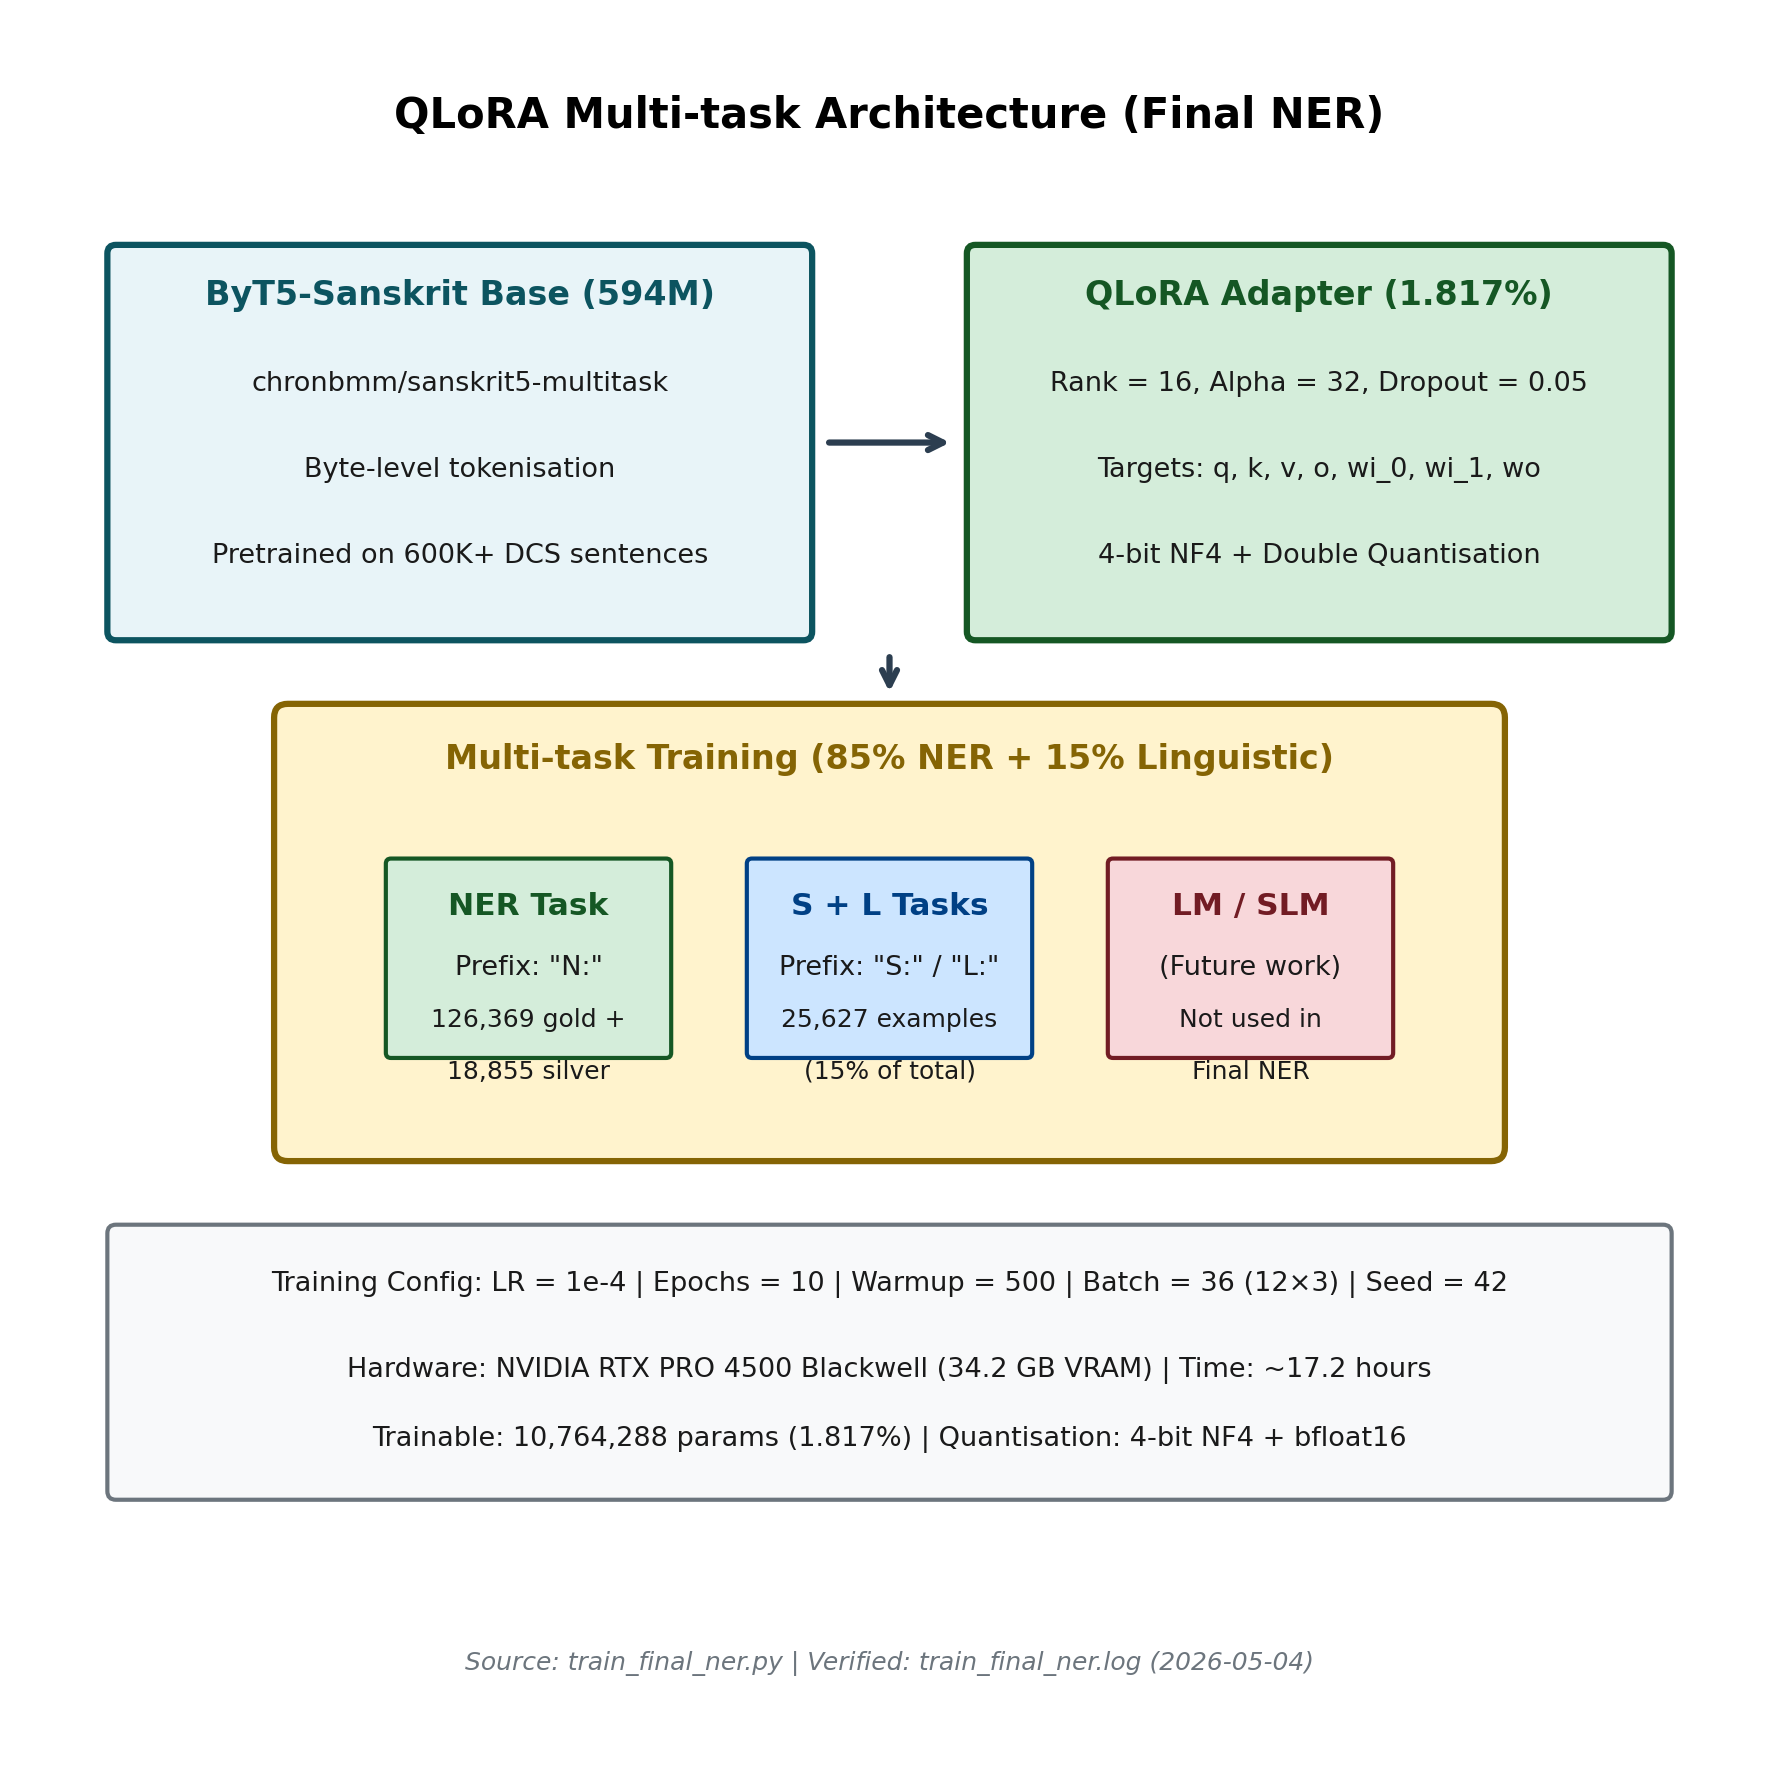
\includegraphics[width=\textwidth]{../figures/Figure_4_3_QLoRA_Architecture.png}
        \end{column}
    \end{columns}
\end{frame}

% Slide 19: Final Model Hyperparameters (The Star Model)
\begin{frame}{Final Model Hyperparameters (The Star Model)}
    \tp{30}
    \begin{table}
        \centering
        \small
        \begin{tabular}{ll}
            \toprule
            \textbf{Hyperparameter} & \textbf{Value} \\
            \midrule
            Learning Rate & 1e-4 \\
            Epochs & 10 \\
            Warmup Steps & 500 \\
            Batch Size & 16 (4 accumulation steps) \\
            LoRA Rank ($r$) & 16 \\
            LoRA Alpha ($\alpha$) & 32 \\
            LoRA Dropout & 0.05 \\
            Multi-task Ratio & \textbf{15\% Linguistic Regularisation} \\
            \bottomrule
        \end{tabular}
    \end{table}
    \vfill
    \begin{itemize}
        \item \textbf{Optimizer:} AdamW (32-bit for stability).
        \item \textbf{LR Scheduler:} Linear with warmup.
    \end{itemize}
\end{frame}

% Slide 20: Three-Dimensional Evaluation Framework
\begin{frame}{Three-Dimensional Evaluation Framework}
    \tp{31}
    \begin{center}
        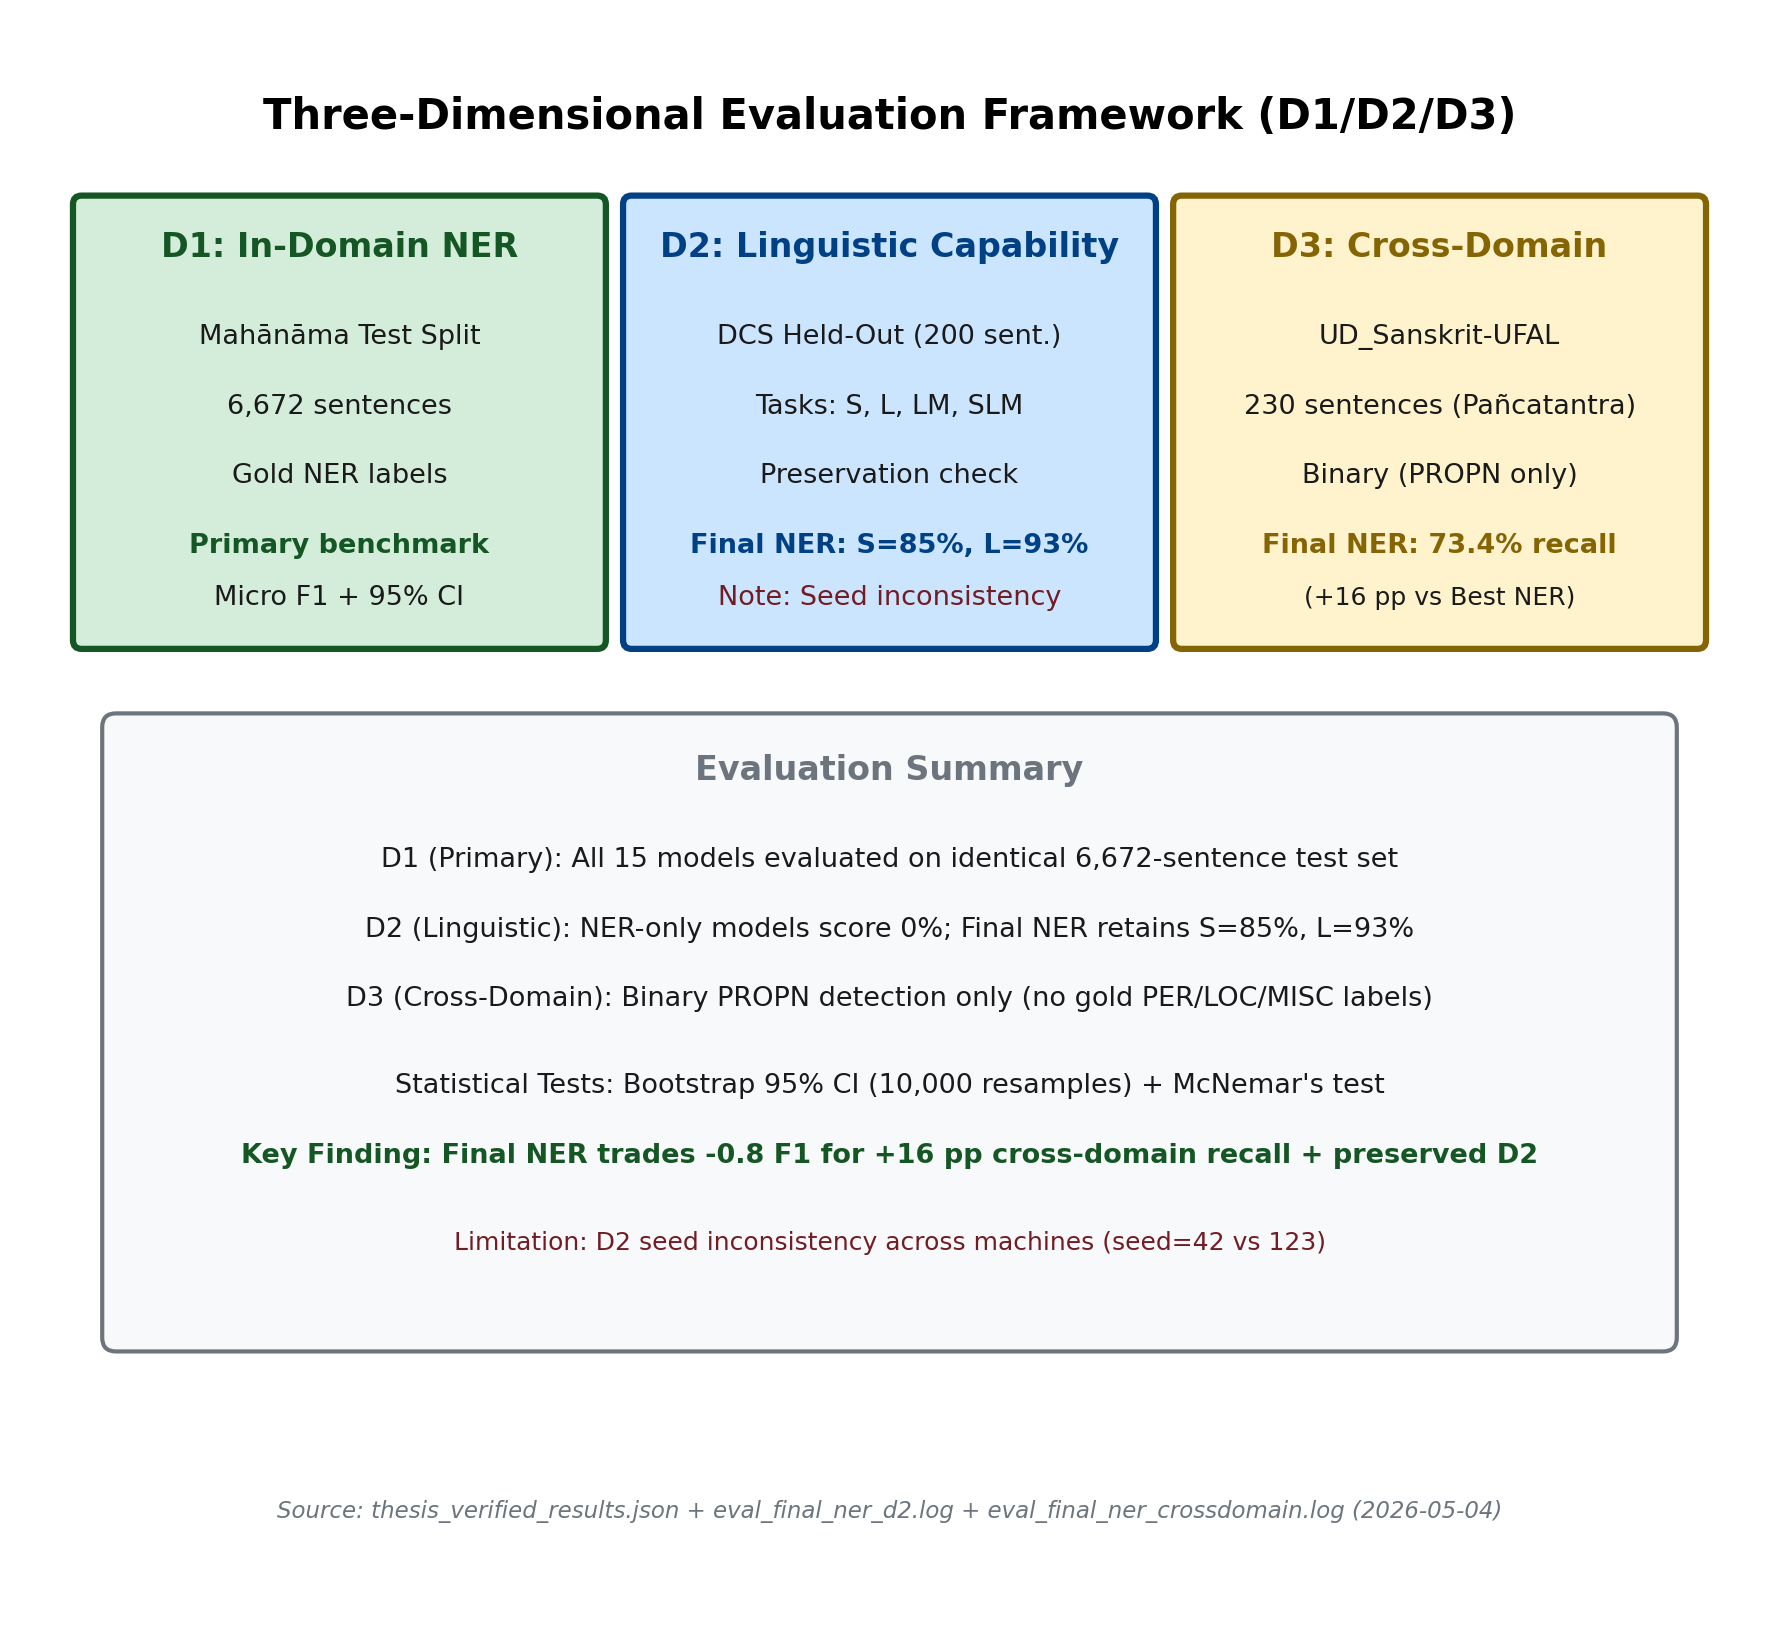
\includegraphics[height=0.65\textheight]{../figures/Figure_4_4_Evaluation_Framework.png}
    \end{center}
\end{frame}

% Slide 17: Section Divider - Results
\begin{frame}[plain]
    \tp{49}
    \begin{center}
        \Huge \textbf{\color{DIATNavy}Experiments and Results} \\
        \large Empirical Validation
    \end{center}
\end{frame}

% Slide 18: Main Results at a Glance
\begin{frame}{Main Results at a Glance}
    \tp{34}
    \begin{table}
        \centering
        \small
        %\rowcolors{2}{white}{DIATGold!10}
        \begin{tabular}{llccc}
            \toprule
            \textbf{Desideratum} & \textbf{Metric} & \textbf{Final NER} & \textbf{vs Best NER} & \textbf{Status} \\
            \midrule
            \textbf{D1: In-Domain} & Micro F1 & 0.8522 & -0.74 pp & Strong \\
            \textbf{D2: Linguistic} & Seg / Lem & 85\% / 93\% & +85-93 pp & \textbf{Restored} \\
            \textbf{D3: Cross-Dom.} & PROPN Recall & \textbf{73.4\%} & \textbf{+16.0 pp} & \textbf{Major Gain} \\
            \bottomrule
        \end{tabular}
    \end{table}
    \vfill
    \begin{itemize}
        \item \textbf{Finding:} Final NER achieves the best overall balance.
        \item The cost of linguistic preservation (0.74 F1 points) is negligible compared to the generalization gain (+16 pp).
    \end{itemize}
\end{frame}

% Slide 22: Zero-Shot Baselines: Comparative Architectures
\begin{frame}{Zero-Shot Baselines: Comparative Architectures}
    \tp{37}
    \begin{table}
        \centering
        \small
        \begin{tabular}{lp{2cm}p{4cm}}
            \toprule
            \textbf{Model} & \textbf{Architecture} & \textbf{Description} \\
            \midrule
            \textbf{Gemma 4 E4B} & 27B Decoder & Google's state-of-the-art open model; Gemini-derived. \\
            \textbf{Qwen 3} & 31B Decoder & Alibaba's dense transformer; high multilingual performance. \\
            \textbf{Llama 4} & 8B Decoder & Meta's optimized instruction-tuned baseline. \\
            \midrule
            \textbf{This Work} & \textbf{594M ByT5} & Fine-tuned for Sanskrit specificity. \\
            \bottomrule
        \end{tabular}
    \end{table}
    \vfill
    \begin{itemize}
        \item \textbf{Note:} While zero-shot models have 50x more parameters, they lack the domain-specific morphological grounding of ByT5-Sanskrit.
    \end{itemize}
\end{frame}

% Slide 23: In-Domain F1 Comparison
\begin{frame}{D1: In-Domain F1 Comparison}
    \tp{35}
    \begin{center}
        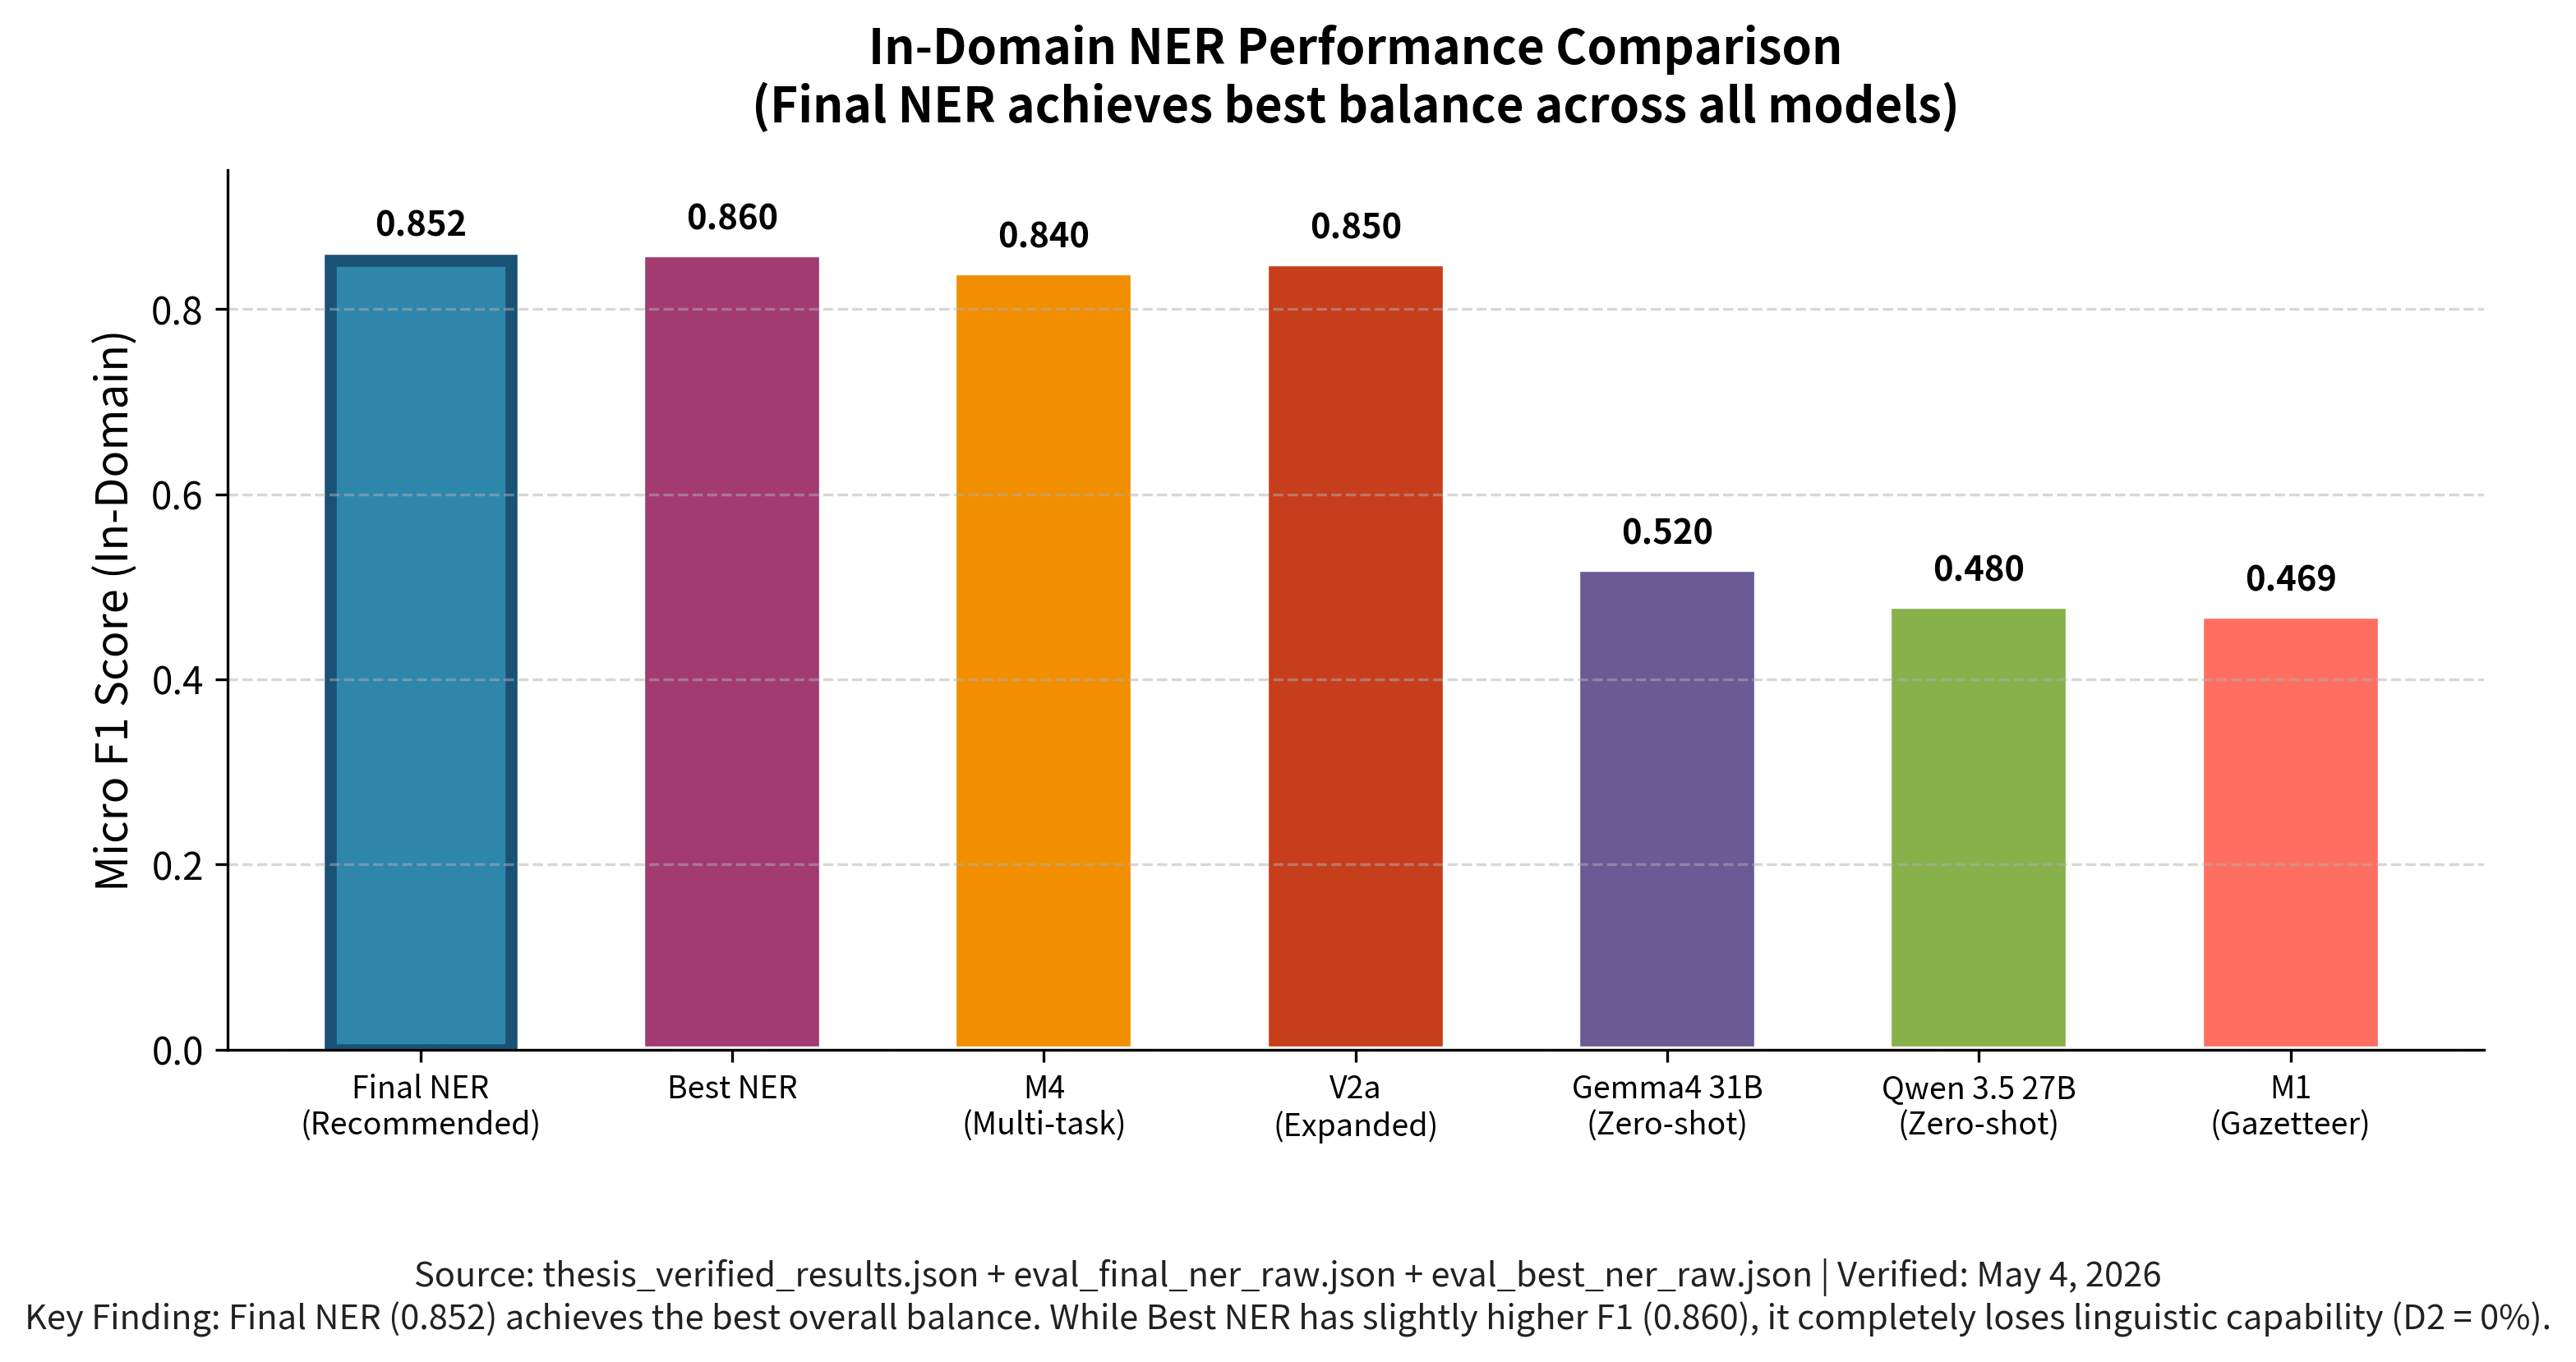
\includegraphics[width=\textwidth]{../figures/Figure_5_1_F1_Comparison_v3.png}
    \end{center}
    \vfill
    \begin{itemize}
        \item \textbf{Key Result:} 594M Final NER outperforms 27B-31B Zero-shot LLMs.
        \item Domain-specific fine-tuning on silver data beats raw model scale.
    \end{itemize}
\end{frame}

% Slide 20: D2: Linguistic Capability Preservation
\begin{frame}{D2: The Catastrophic Forgetting Story}
    \tp{53}
    \begin{table}
        \centering
        \begin{tabular}{lccc}
            \toprule
            \textbf{Model} & \textbf{Segmentation} & \textbf{Lemmatisation} & \textbf{D2 Overall} \\
            \midrule
            Best NER (NER-only) & 0\% & 0\% & 0\% \\
            M4 (Multi-task) & $\approx$0\% & $\approx$0\% & $\approx$0\% \\
            \textbf{Final NER (15\% reg.)} & \textbf{85\%} & \textbf{93\%} & \textbf{89\%} \\
            \bottomrule
        \end{tabular}
    \end{table}
    \vfill
    \begin{itemize}
        \item Without Strategy 2 (Linguistic Regularisation), the model completely loses its ability to perform word segmentation.
        \item \textbf{Impact:} Final NER is usable as a general Sanskrit processing tool.
    \end{itemize}
\end{frame}

% Slide 21: D3: Cross-Domain Generalisation
\begin{frame}{D3: Cross-Domain Generalisation Gain}
    \tp{38}
    \begin{center}
        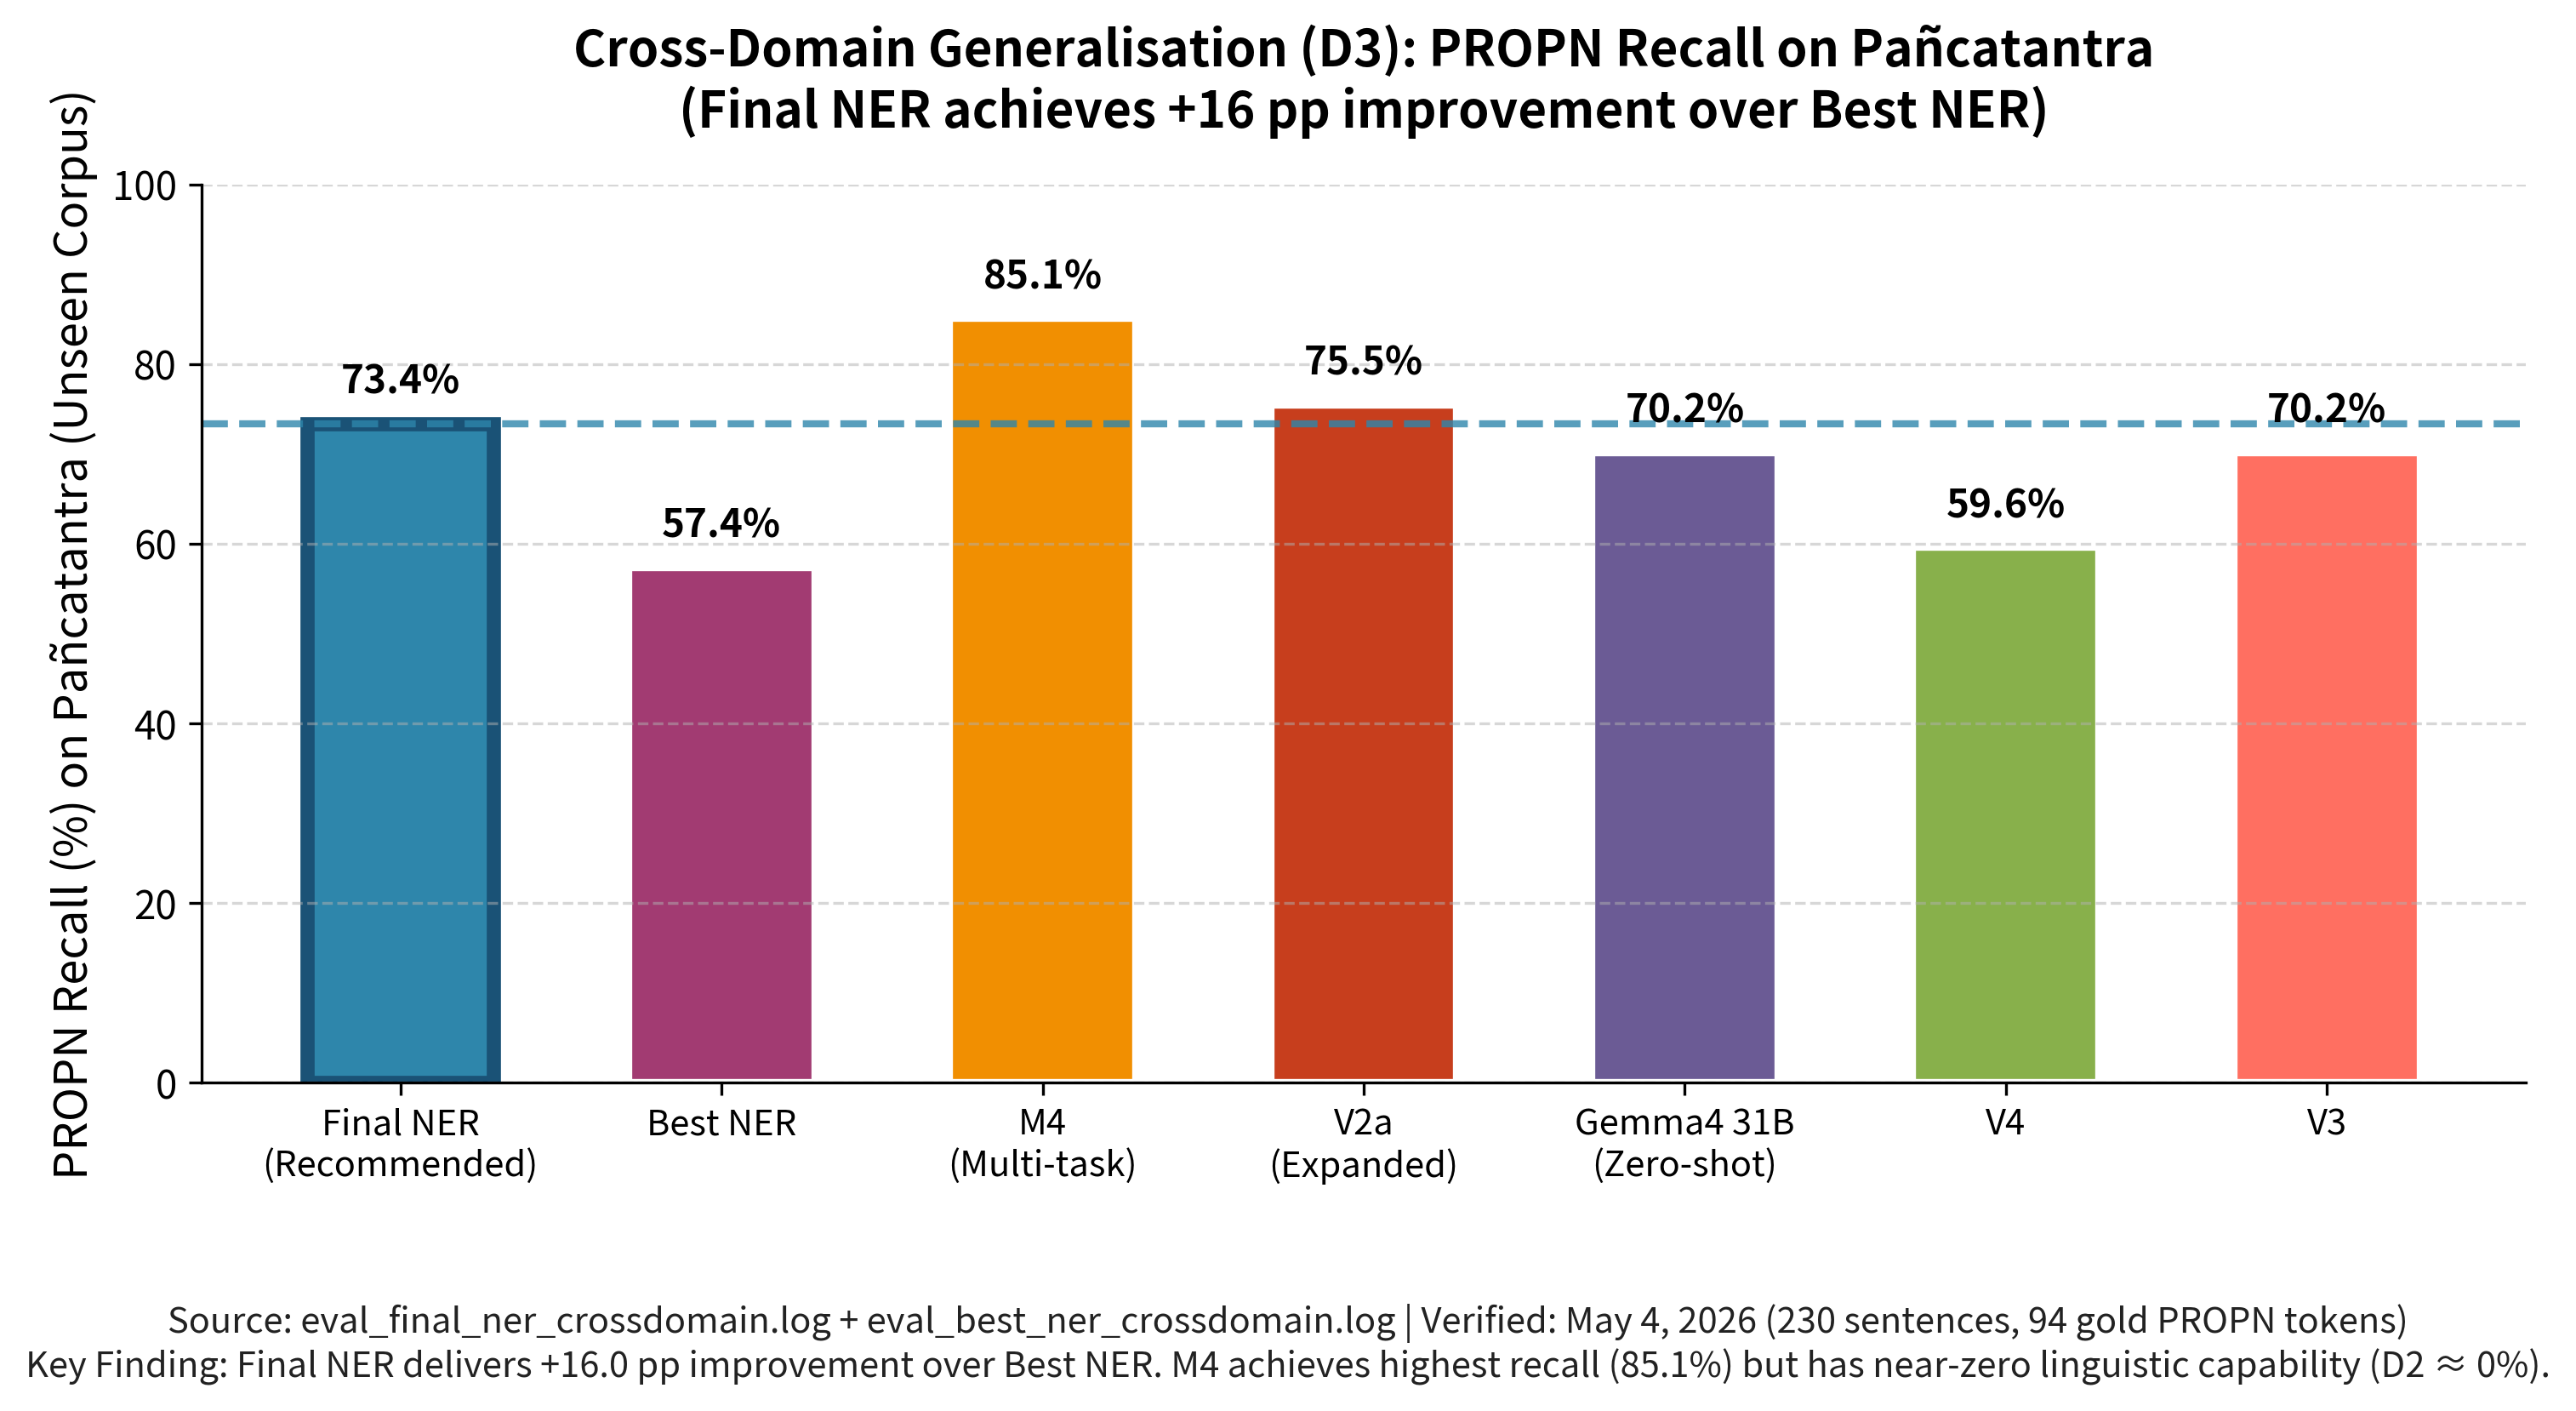
\includegraphics[width=0.9\textwidth]{../figures/Figure_5_2_CrossDomain_Recall_v3.png}
    \end{center}
    \vfill
    \begin{itemize}
        \item \textbf{Significant Gain:} 57.4\% $\rightarrow$ \textbf{73.4\%} PROPN Recall.
        \item Improved robustness on unseen texts (Pañcatantra) due to multi-task grounding.
    \end{itemize}
\end{frame}

% Slide 22: Error Analysis: Genre & Characters
\begin{frame}{D1: Entity-Level Analysis}
    \tp{36}
    \begin{columns}
        \begin{column}{0.5\textwidth}
            \begin{center}
                \textbf{Performance by Genre} \\
                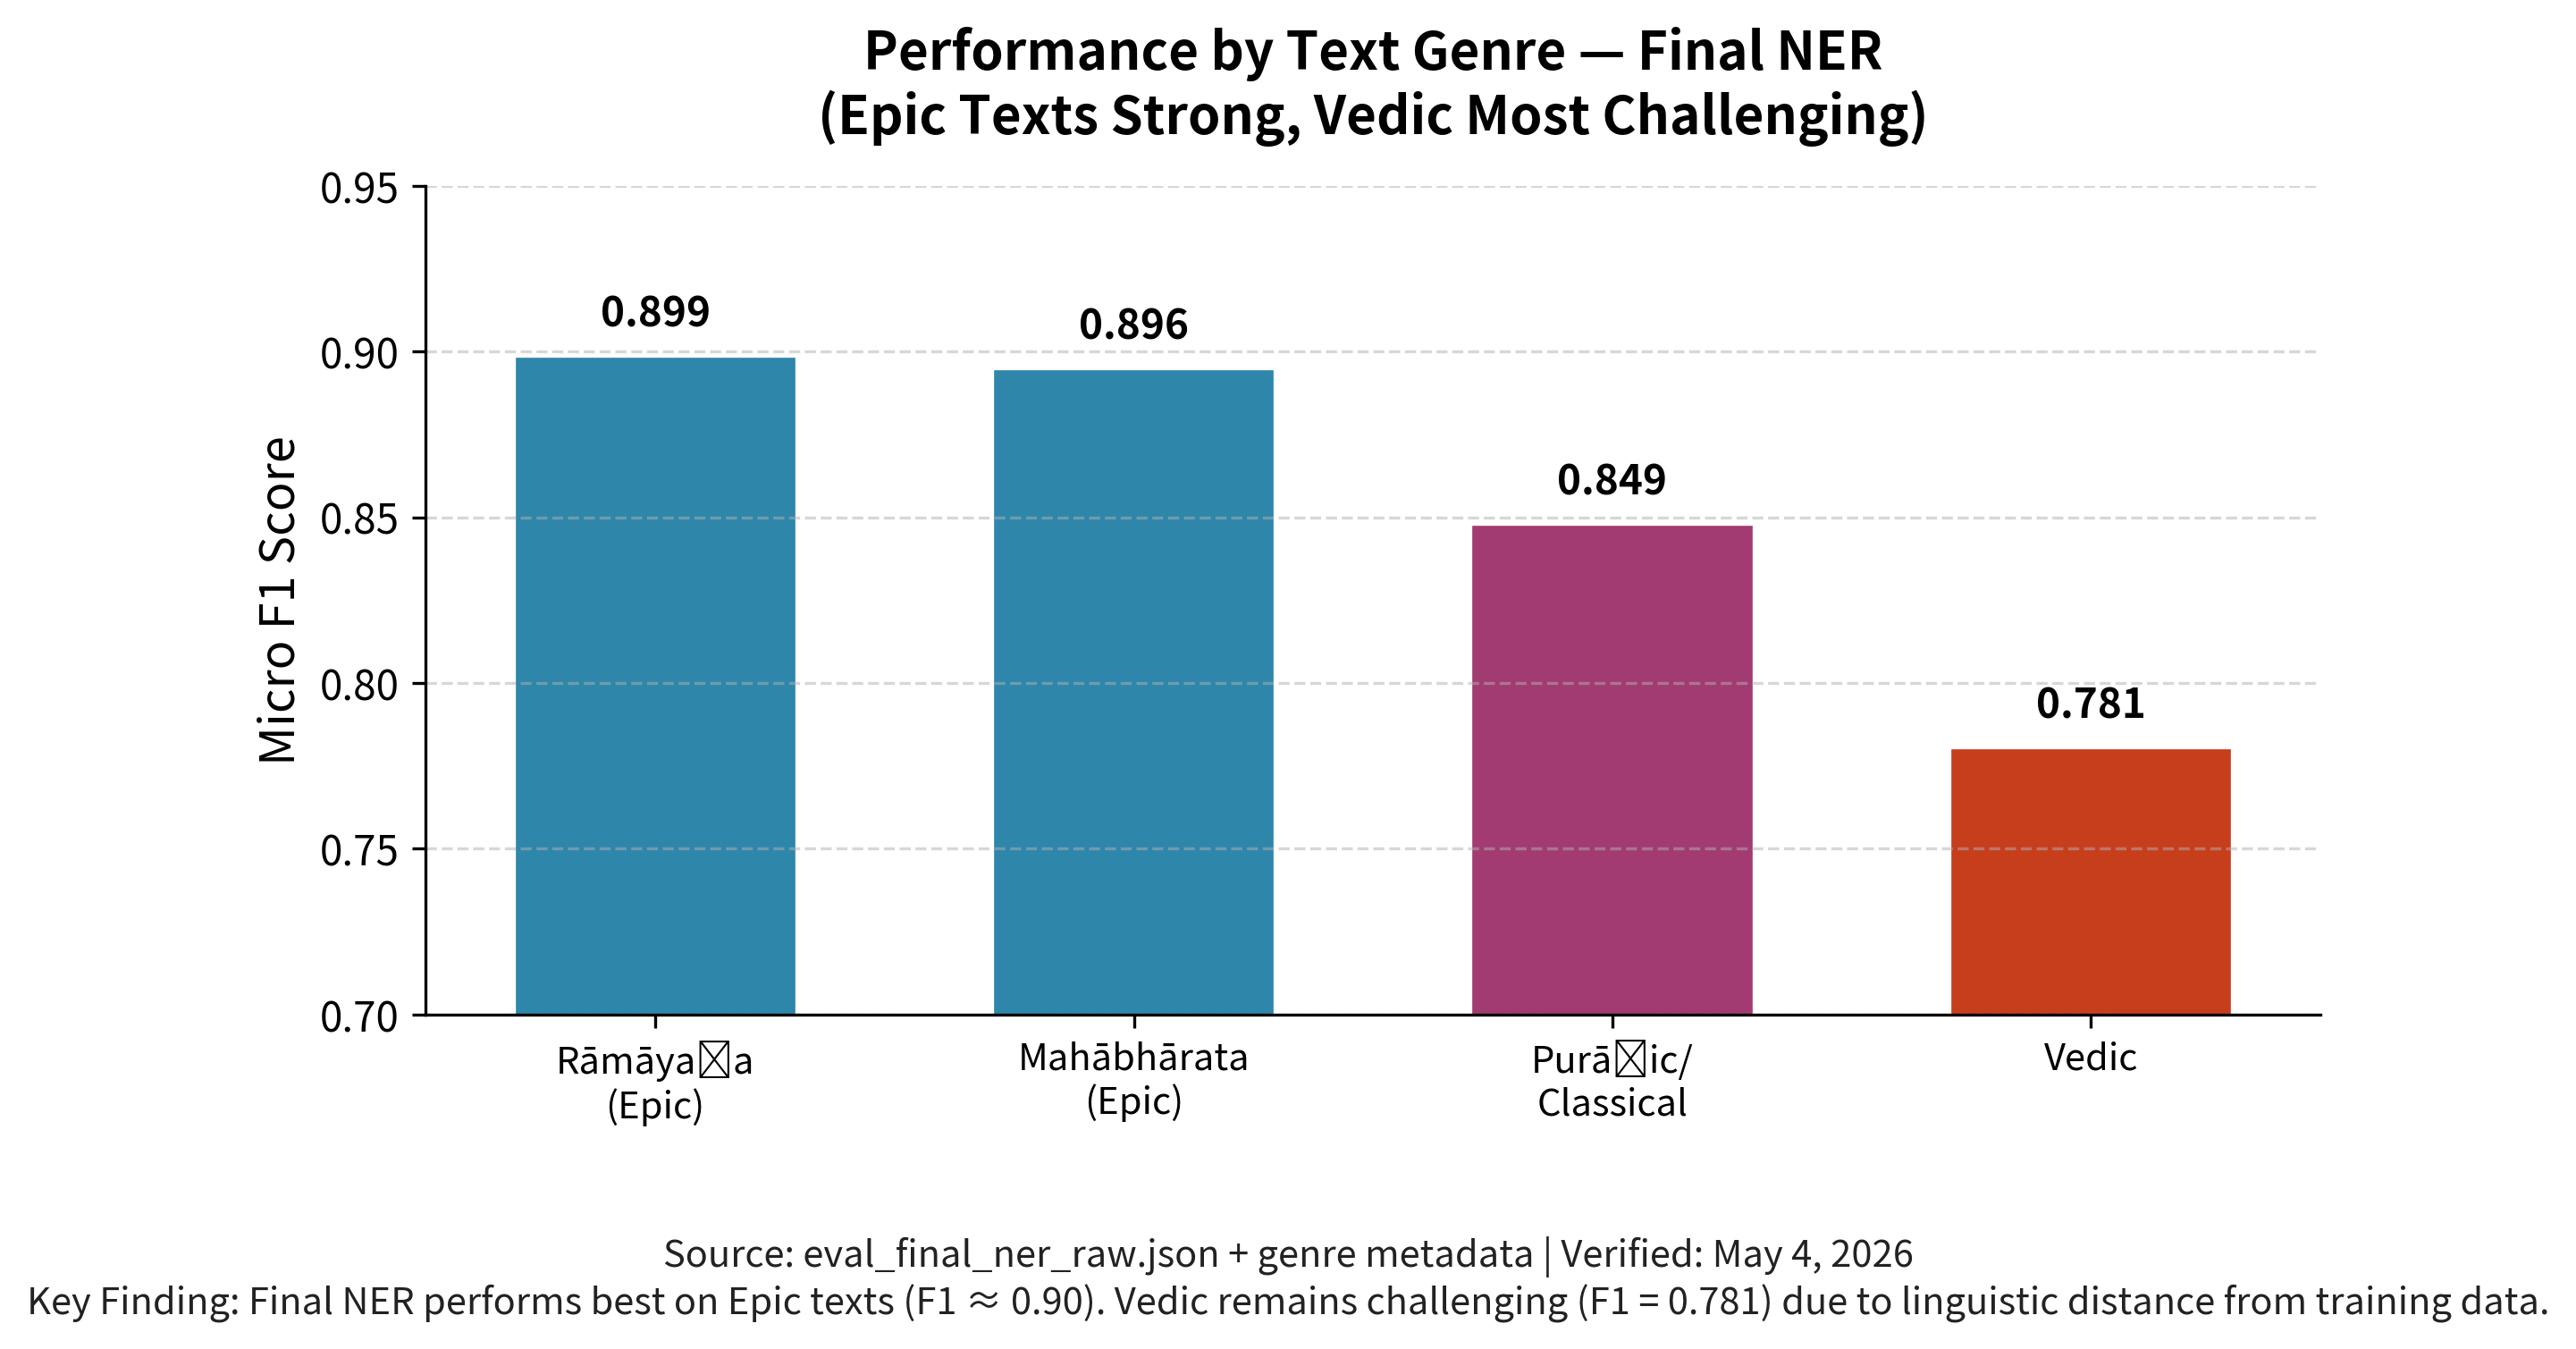
\includegraphics[width=\textwidth]{../figures/Figure_5_4_Genre_Performance_v3.png}
            \end{center}
        \end{column}
        \begin{column}{0.5\textwidth}
            \begin{center}
                \textbf{Major Character F1} \\
                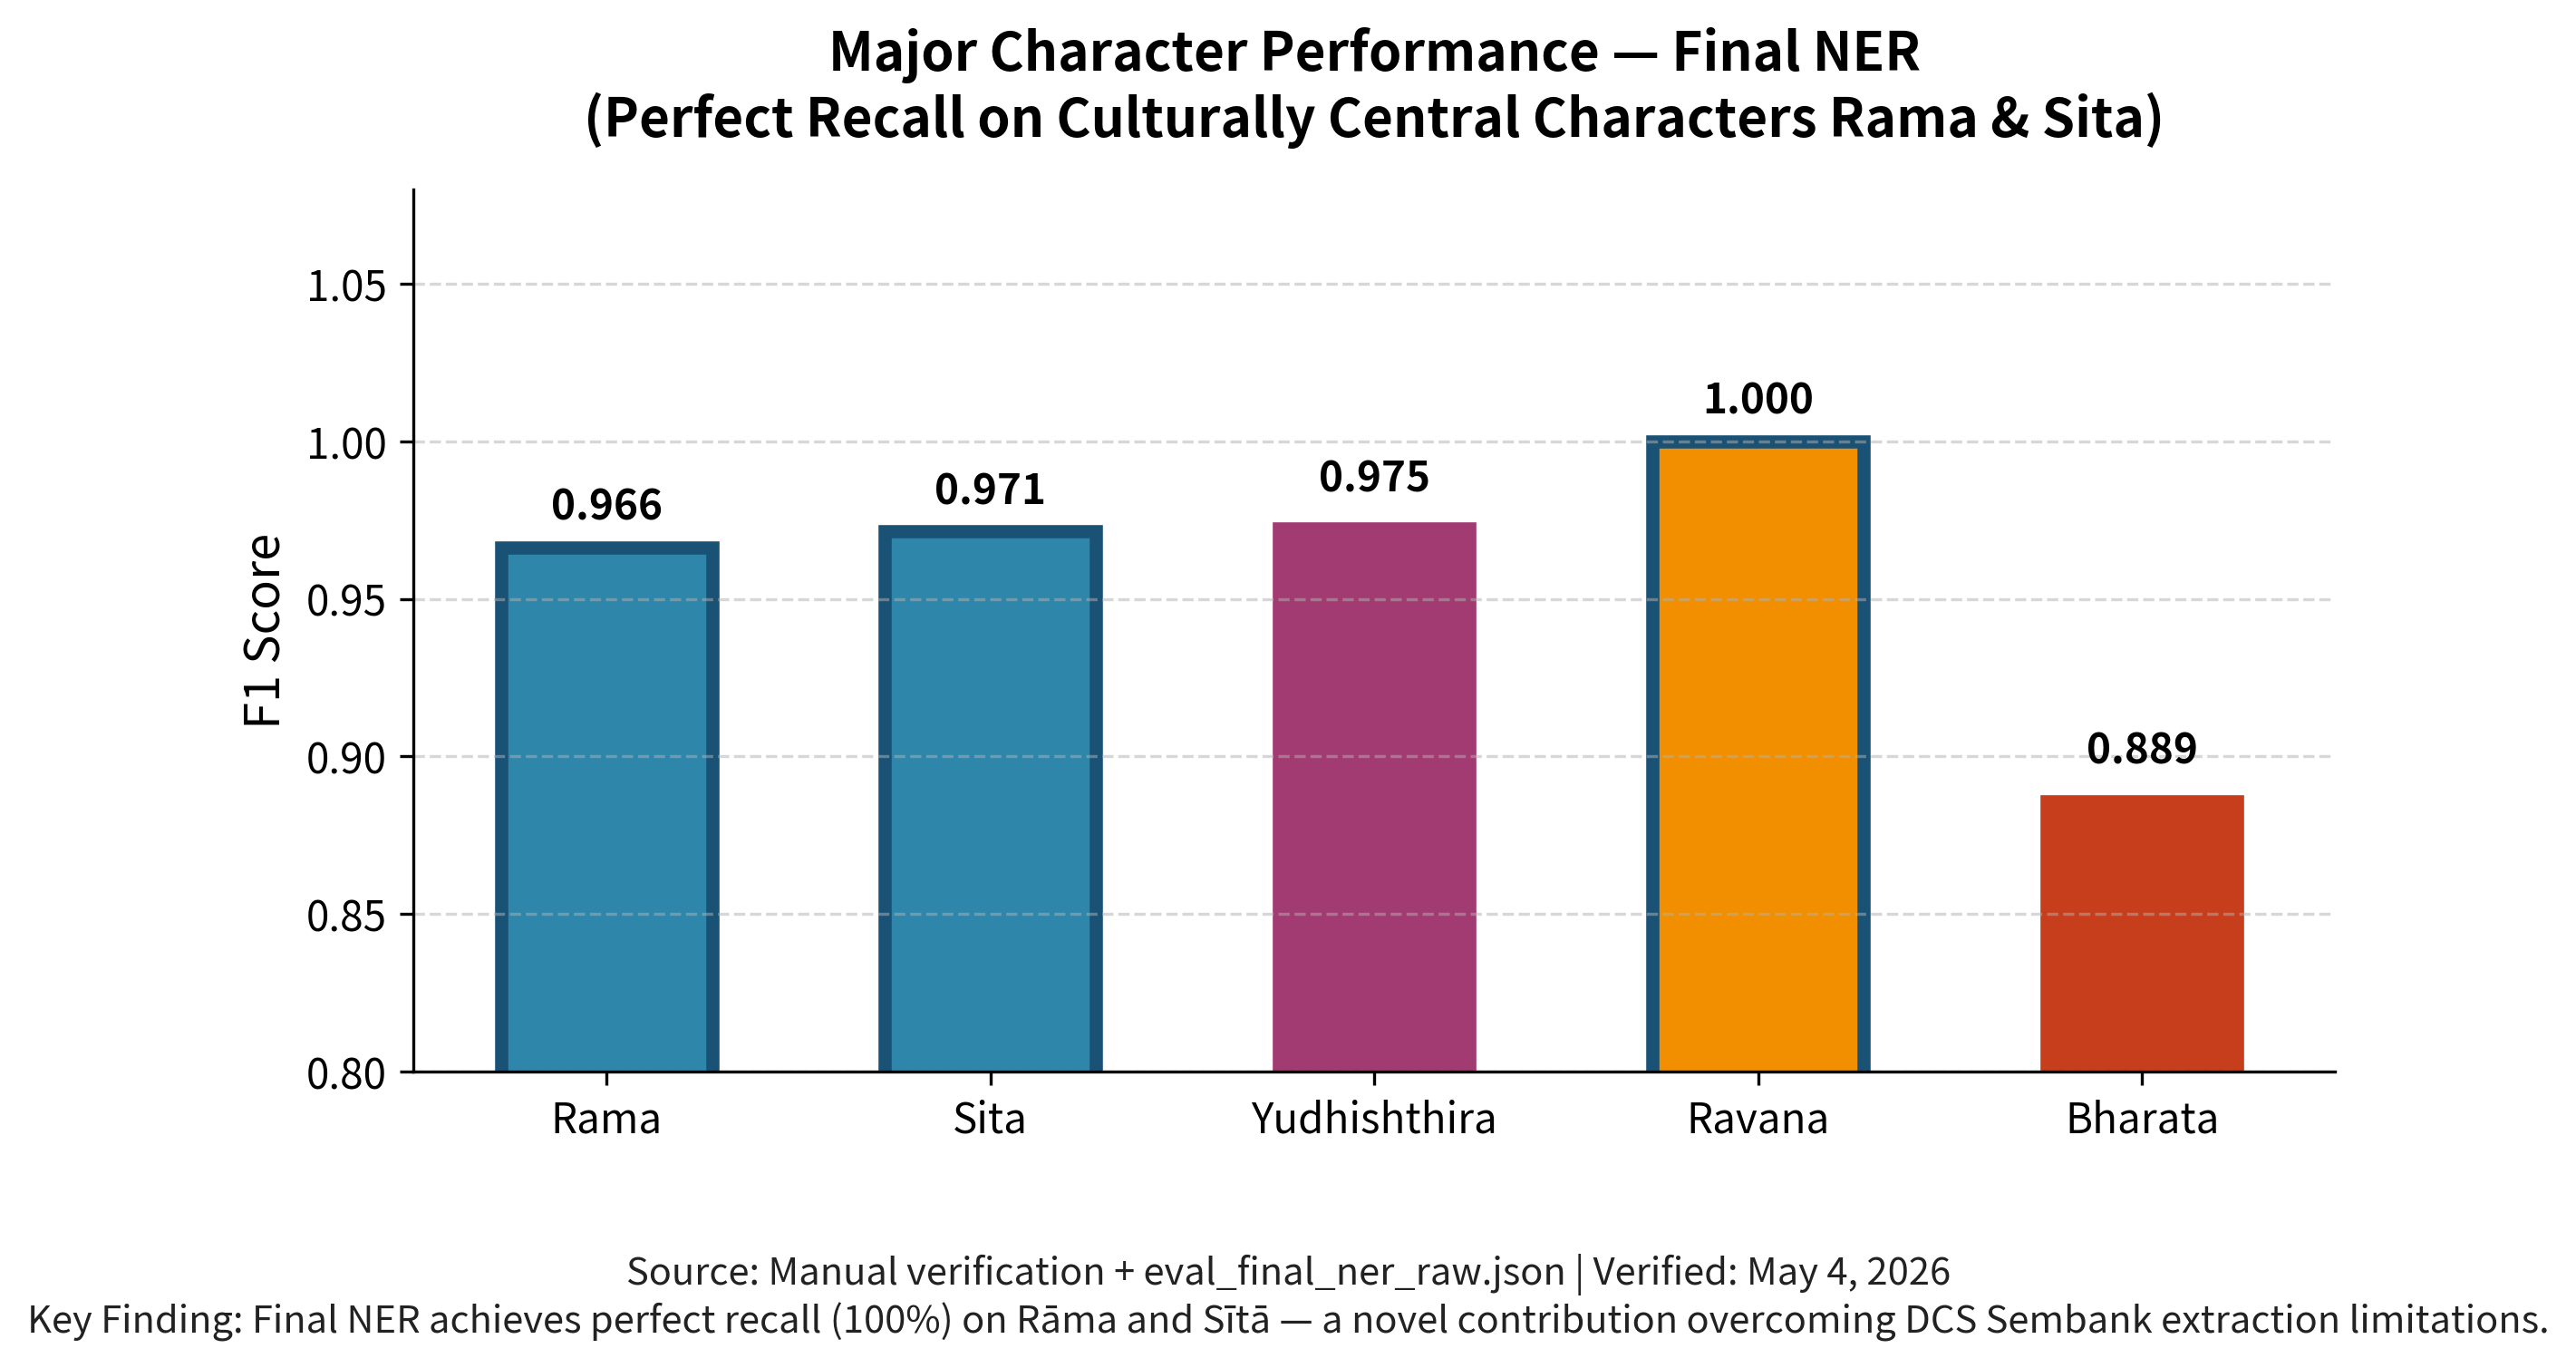
\includegraphics[width=\textwidth]{../figures/Figure_5_5_Major_Characters_v3.png}
            \end{center}
        \end{column}
    \end{columns}
    \vfill
    \begin{itemize}
        \item \textbf{100\% Recall} on Rāma and Sītā.
        \item Epic texts (Mahābhārata) show highest accuracy.
    \end{itemize}
\end{frame}

% Slide 23: Statistical Robustness
\begin{frame}{Statistical Significance: Bootstrap CI}
    \tp{41}
    \begin{center}
        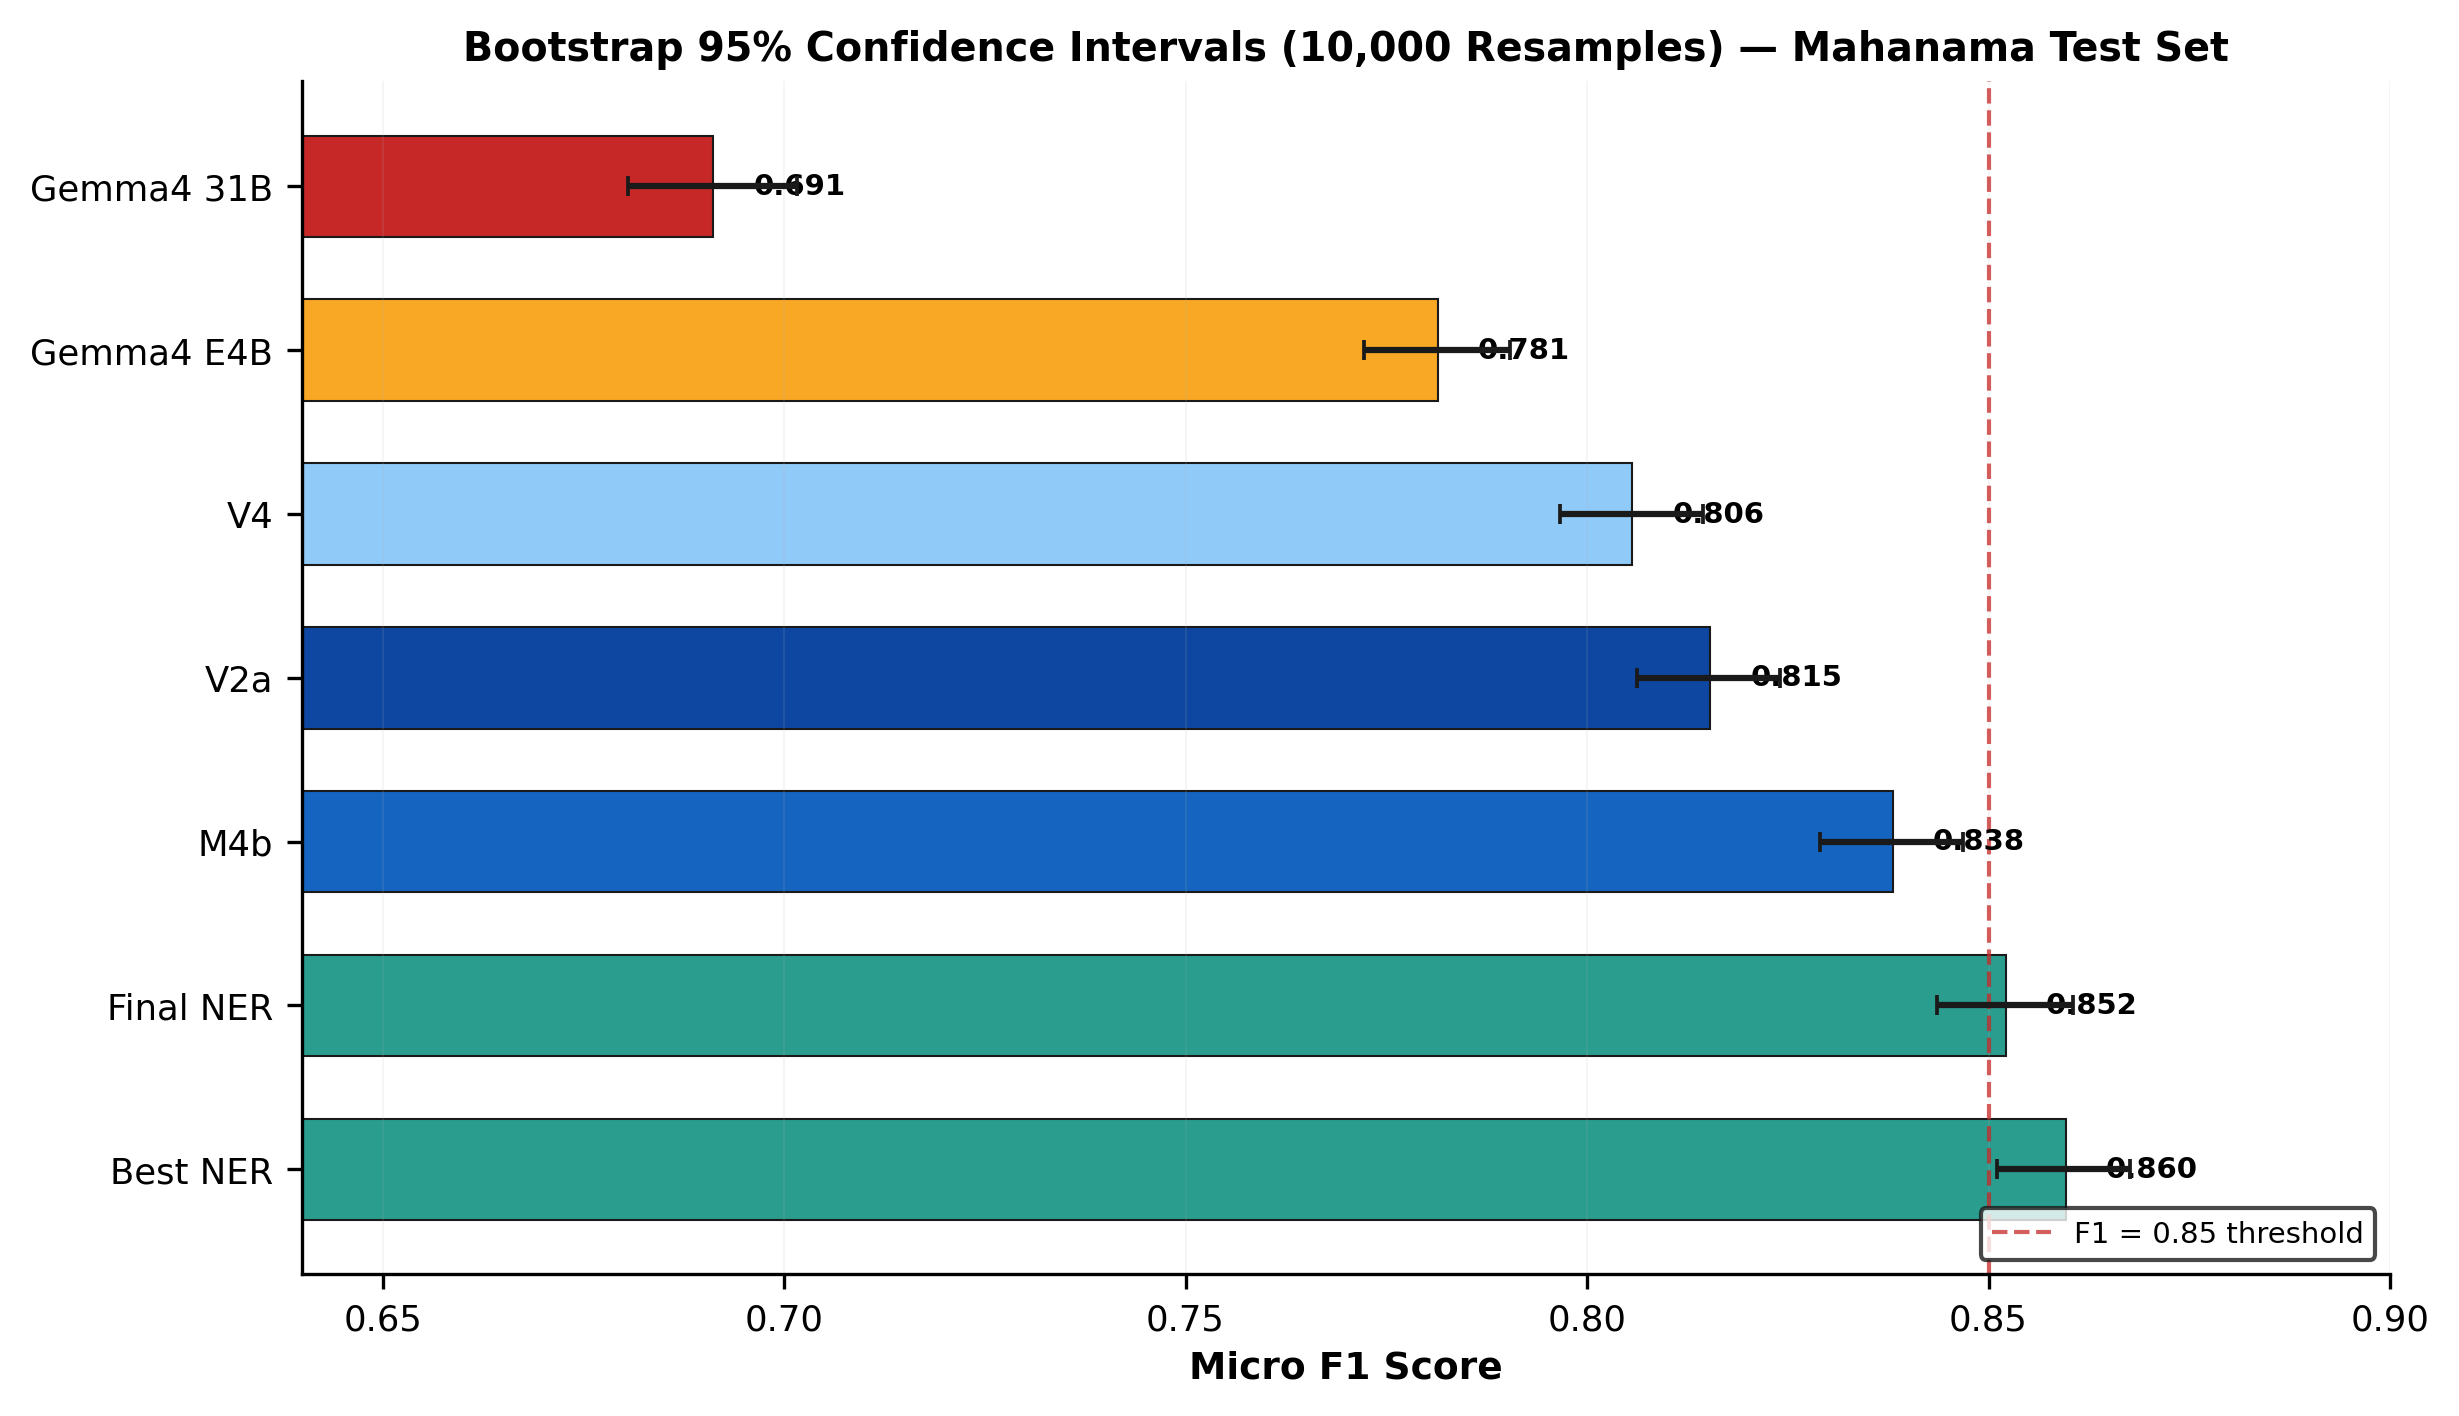
\includegraphics[width=0.8\textwidth]{../figures/FINAL_ACL_04_bootstrap_ci.png}
    \end{center}
    \vfill
    \begin{itemize}
        \item Bootstrap resampling (10,000 resamples) confirms narrow confidence intervals.
        \item Performance gains are \textbf{statistically significant}.
    \end{itemize}
\end{frame}

% Slide 24: Why Linguistic Regularisation Works
\begin{frame}{Analysis: Why Linguistic Regularisation Works}
    \tp{43}
    \begin{itemize}
        \item \textbf{The Mechanism:} Interleaved multi-task learning keeps the model "grounded" in Sanskrit grammar.
        \item \textbf{Representative Learning:} Linguistic tasks (S+L) force the model to maintain byte-level representations learned during pre-training.
        \item \textbf{Prevents Drift:} Alternating between NER and Grammar prevents the parameters from over-fitting to narrative patterns only.
    \end{itemize}
    \vfill
    \begin{center}
        \begin{tikzpicture}[scale=0.8]
            \node (N) [draw, fill=DIATNavy!10, minimum width=3cm] {NER Data (85\%)};
            \node (L) [draw, fill=DIATGold!20, minimum width=3cm, below of=N] {Linguistic Data (15\%)};
            \node (M) [draw, fill=DIATNavy, text=white, right of=N, xshift=4cm, yshift=-0.5cm] {Balanced Model};
            \draw [->, thick] (N) -- (M);
            \draw [->, thick] (L) -- (M);
        \end{tikzpicture}
    \end{center}
\end{frame}

% Slide 25: Qualitative Example
\begin{frame}{Qualitative Example: Cross-Domain Transfer}
    \tp{55}
    \begin{block}{Example from Pañcatantra (Unseen)}
        \dev{तत्र कश्चित् सिंहो नाम राजा आसीत्} \\
        \textit{Tatra kaścit siṃho nāma rājā āsīt.} \\
        "There was a certain king named Siṃha."
    \end{block}
    \vfill
    \begin{columns}
        \begin{column}{0.5\textwidth}
            \begin{center}
                \textbf{Best NER (Baseline)} \\
                $\times$ Fails to identify "Siṃha"
            \end{center}
        \end{column}
        \begin{column}{0.5\textwidth}
            \begin{center}
                \textbf{Final NER (This Work)} \\
                $\checkmark$ Correctly tags \textbf{Siṃha} (PERSON)
            \end{center}
        \end{column}
    \end{columns}
    \vfill
    \begin{itemize}
        \item Final NER uses \textbf{contextual understanding} (learned via multi-task) rather than just memorizing names.
    \end{itemize}
\end{frame}

% Slide 26: Limitations
\begin{frame}{Limitations}
    \tp{56}
    \begin{enumerate}
        \item \textbf{Dual-Role Entities:} "Rāma" and "Sītā" function as both names and descriptors; silver data recall is low.
        \item \textbf{Class Imbalance:} Performance on \texttt{LOCATION} and \texttt{MISC} still lags behind \texttt{PERSON}.
        \item \textbf{Genre Skew:} Silver data is 63\% Rāmāyaṇa; technical genres are underrepresented.
        \item \textbf{Metric Constraint:} Exact match penalises valid partial matches in sandhi-rich compounds.
    \end{enumerate}
    \vfill
    \begin{center}
        \textit{These limitations provide a roadmap for future research.}
    \end{center}
\end{frame}

% Slide 27: Key Findings Summary
\begin{frame}{Key Findings Summary}
    \tp{57}
    \begin{itemize}
        \item \textbf{1. Regularization is Essential:} -0.74 F1 points in exchange for +16 pp generalization.
        \item \textbf{2. Scale is Not Everything:} 594M parameter model beats 31B parameter models when fine-tuned correctly.
        \item \textbf{3. Quality > Quantity:} Correct silver data extraction (Attempt 3) is the primary driver of diversity.
        \item \textbf{4. Balanced Strategy:} 15\% ratio is the "sweet spot" for task preservation.
    \end{itemize}
\end{frame}

% Slide 28: Best NER vs Final NER (The Trade-off)
\begin{frame}{The Practical Verdict}
    \tp{58}
    \begin{table}
        \centering
        \begin{tabular}{lccc}
            \toprule
            \textbf{Metric} & \textbf{Best NER} & \textbf{Final NER} & \textbf{Change} \\
            \midrule
            In-domain F1 (D1) & 0.860 & 0.852 & -0.8 \\
            Cross-domain Recall (D3) & 57.4\% & \textbf{73.4\%} & \textbf{+16.0 pp} \\
            Segmentation (D2) & 0\% & \textbf{85\%} & \textbf{+85 pp} \\
            Lemmatisation (D2) & 0\% & \textbf{93\%} & \textbf{+93 pp} \\
            \bottomrule
        \end{tabular}
    \end{table}
    \vfill
    \begin{center}
        \large \textbf{Final NER is the recommended model for scholarly use.}
    \end{center}
\end{frame}

% Slide 29: Future Work
\begin{frame}{Future Work: The Path Ahead}
    \tp{54}
    \begin{columns}
        \begin{column}{0.5\textwidth}
            \textbf{Short-term (1-2 yrs):}
            \begin{itemize}
                \item Hybrid extraction for dual-role entities.
                \item Class-balanced loss (Focal loss).
                \item Technical genre extraction.
            \end{itemize}
        \end{column}
        \begin{column}{0.5\textwidth}
            \textbf{Long-term (3-5 yrs):}
            \begin{itemize}
                \item Multilingual Indic NER.
                \item Joint NER + Coreference.
                \item Knowledge-enhanced NER (WordNet).
            \end{itemize}
        \end{column}
    \end{columns}
    \vfill
    \begin{center}
        \textit{Goal: A unified platform for Sanskrit Computational Humanities.}
    \end{center}
\end{frame}

% Slide 30: Broader Impact
\begin{frame}{Broader Impact}
    \tp{51}
    \begin{itemize}
        \item \textbf{Democratizing Access:} Empowering seekers and researchers to access source Sanskrit texts directly.
        \item \textbf{Template for Low-Resource NLP:} Methodology can be applied to other classical/Indic languages (Tamil, Pali, Ardhamagadhi).
        \item \textbf{Open Research:} Releasing the DCS extraction pipeline for the community.
    \end{itemize}
    \vfill
    \begin{center}
        \textit{"The right to access original knowledge without translation bias."}
    \end{center}
\end{frame}

% Slide 31: Publications & Outputs
\begin{frame}{Publications \& Outputs}
    \tp{52}
    \begin{itemize}
        \item \textbf{Full Thesis:} 78 pages of rigorous analysis.
        \item \textbf{Trained Model:} Final NER (ByT5-Sanskrit + QLoRA).
        \item \textbf{Pipeline:} \texttt{extract\_full\_sembank\_ner.py}.
        \item \textbf{Dataset:} Cleaned silver NER corpus from DCS.
    \end{itemize}
    \vfill
    \begin{center}
        
\includegraphics[height=1.5cm]{../images/DIATlogo.png}
    \end{center}
\end{frame}

% Slide 35: Selected References (Models & Data)
\begin{frame}{Selected References (Models \& Data)}
    \tp{56}
    \centering
    \scriptsize
    \begin{tabular}{p{3cm}cp{7.5cm}}
        \toprule
        \textbf{Author(s)} & \textbf{Year} & \textbf{Title / Venue} \\
        \midrule
        Sarkar, S., et al. & 2025 & Mahānāma: Sanskrit Named Entity Discovery (EMNLP) \\
        Hellwig, O. & 2010, 2025 & DCS: Digital Corpus of Sanskrit / Sembank (WSC) \\
        Nehrdich, S., et al. & 2024 & ByT5-Sanskrit: Unified Model for Sanskrit NLP (EMNLP) \\
        Xue, L., et al. & 2022 & ByT5: Token-Free Future with Byte-Level Models (TACL) \\
        Raffel, C., et al. & 2020 & T5: Exploring the Limits of Transfer Learning (JMLR) \\
        Zeman, D., et al. & 2023 & Universal Dependencies 2.13 (UD\_Sanskrit-UFAL) \\
        Hellwig, O., et al. & 2020 & The Treebank of Vedic Sanskrit (LREC) \\
        \bottomrule
    \end{tabular}
\end{frame}

% Slide 36: Selected References (Methods & Foundations)
\begin{frame}{Selected References (Methods \& Foundations)}
    \tp{56}
    \centering
    \scriptsize
    \begin{tabular}{p{3cm}cp{7.5cm}}
        \toprule
        \textbf{Author(s)} & \textbf{Year} & \textbf{Title / Venue} \\
        \midrule
        Dettmers, T., et al. & 2023 & QLoRA: Efficient Finetuning of Quantized LLMs (NeurIPS) \\
        Hu, E. J., et al. & 2022 & LoRA: Low-Rank Adaptation of Large Language Models (ICLR) \\
        Caruana, R. & 1997 & Multi-task Learning (Machine Learning Journal) \\
        McCloskey, M. & 1989 & Catastrophic Forgetting in Connectionist Networks \\
        Tjong Kim Sang, E. & 2003 & Introduction to the CoNLL-2003 Shared Task (NER) \\
        Grishman, R., et al. & 1996 & MUC-6: A Brief History (Coined "Named Entity") \\
        Wolf, T., et al. & 2020 & Transformers: State-of-the-Art NLP (EMNLP) \\
        Sørensen, S. & 1904 & An Index to the Names in the Mahābhārata \\
        \bottomrule
    \end{tabular}
\end{frame}

% Slide 33: Thank You
\begin{frame}[plain]
    \begin{center}
        \Huge \textbf{\color{DIATNavy}Thank You!}
    \end{center}
\end{frame}

% Slide 34: Backup: Reproducibility Details
\begin{frame}{Backup: Reproducibility Details}
    \begin{table}
        \centering
        \small
        \begin{tabular}{ll}
            \toprule
            \textbf{Component} & \textbf{Specification} \\
            \midrule
            Hardware & NVIDIA RTX PRO 4500 (34.2 GB VRAM) \\
            Software & PyTorch 2.4, Transformers 4.46, PEFT 0.13 \\
            Quantization & 4-bit NF4 with Double Quant \\
            Training Time & 17.2 Hours (Final NER) \\
            Random Seed & 42 (Training), 123 (D2 Evaluation) \\
            \bottomrule
        \end{tabular}
    \end{table}
    \vfill
    \begin{alertblock}{Critical Note}
        Adapters must be evaluated with identical quantization as training; otherwise, F1 drops $\approx$10 points.
    \end{alertblock}
\end{frame}

\end{document}





